%%% Sekce - Návrh produktu
%%%%% Wording: ✅
%%%%% Styling: ✅
%%%%% References: ✅
%%%%% Grammar: ✅
%%% --------------------------------------------------------------
\section{Návrh produktu}
\label{sec:navrh-ui-navrh-produktu}
\acl{ui} a \acl{ux} jsou oba úzce spjaty s pochopením potřeb uživatele.
Když je produkt navrhován, není vždy okamžitě jasné, jakým způsobem by mělo být jeho uživatelské rozhraní vypadat.
Uživatelské příběhy, pokud jsou správně navrženy, usnadňují spojení mezi potřebami uživatele a strukturální kompozicí produktu.
Primárním cílem je v této sekci přetvořit výše navržené uživatelské příběhy do \ac{ui} jednotlivých komponent uživatelského rozhraní, které nakonec utvoří interaktivní architekturu produktu.

\ac{ui} komponenty jsou prvky, které tvoří interaktivní a vizuální aspekty uživatelského rozhraní produktu.
Tyto komponenty mohou zahrnovat menší jednodušší designové prvky, jako jsou například tlačítka či ikony, nebo větší a složitější funkční jednotky, jako je ku příkladu navigační menu nebo interaktivní plánek sedaček.

Převedení uživatelských příběhů do \ac{ui} komponent je klíčovým krokem tomto v procesu, který vyžaduje hluboké porozumění potřebám uživatele tak, jak jsou vyjádřeny v uživatelských příbězích, a schopnost vizualizovat, jak tyto potřeby mohou být zhmotněny prostřednictvím různých \ac{ui} komponent.
Pro produkt, jako je aplikace na prodej vstupenek, to znamená zaměřit se na komponenty, které umožňují uživatelům navigovat po interaktivním plánu sedadel, vybrat si svá požadovaná místa a dokončit nákup vstupenek s minimálním distrakcí a maximální jednoduchostí.

Tato kapitola se dále zaměří na proces převodu výše sestrojených uživatelských příběhů do konkrétních \ac{ui} komponent, které budou tvořit výsledný návrh uživatelského rozhraní vyvíjené webové aplikace.

%%% Podsekce - Vizualizace místa konání
%%%%% Wording: ✅
%%%%% Styling: ✅
%%%%% References: ✅
%%%%% Grammar: ✅
%%% --------------------------------------------------------------
\begin{subsection}{Vizualizace místa konání}
    \label{subsec:narvh-ui-transformace-uzivatelskych-pribehu-vizualizace-mista-konani}
    \userstoryvenuemap

    Základní myšlenkou tohoto příběhu je, že by uživatelé měli mít možnost zobrazit plán sedadel místa konání, aby mohli snadno vybrat svá preferovaná místa.
    To znamená navržení komplexní komponenty, která bude tuto funkčnost zajišťovat.
    Tato komponenta by měla být schopna zobrazit plán sedadel místa konání, který bude obsahovat sedadla a případné další objekty umístěné v místě konání.

    \begin{figure}[H]
        \centering
        \begin{subfigure}{0.775\textwidth}
            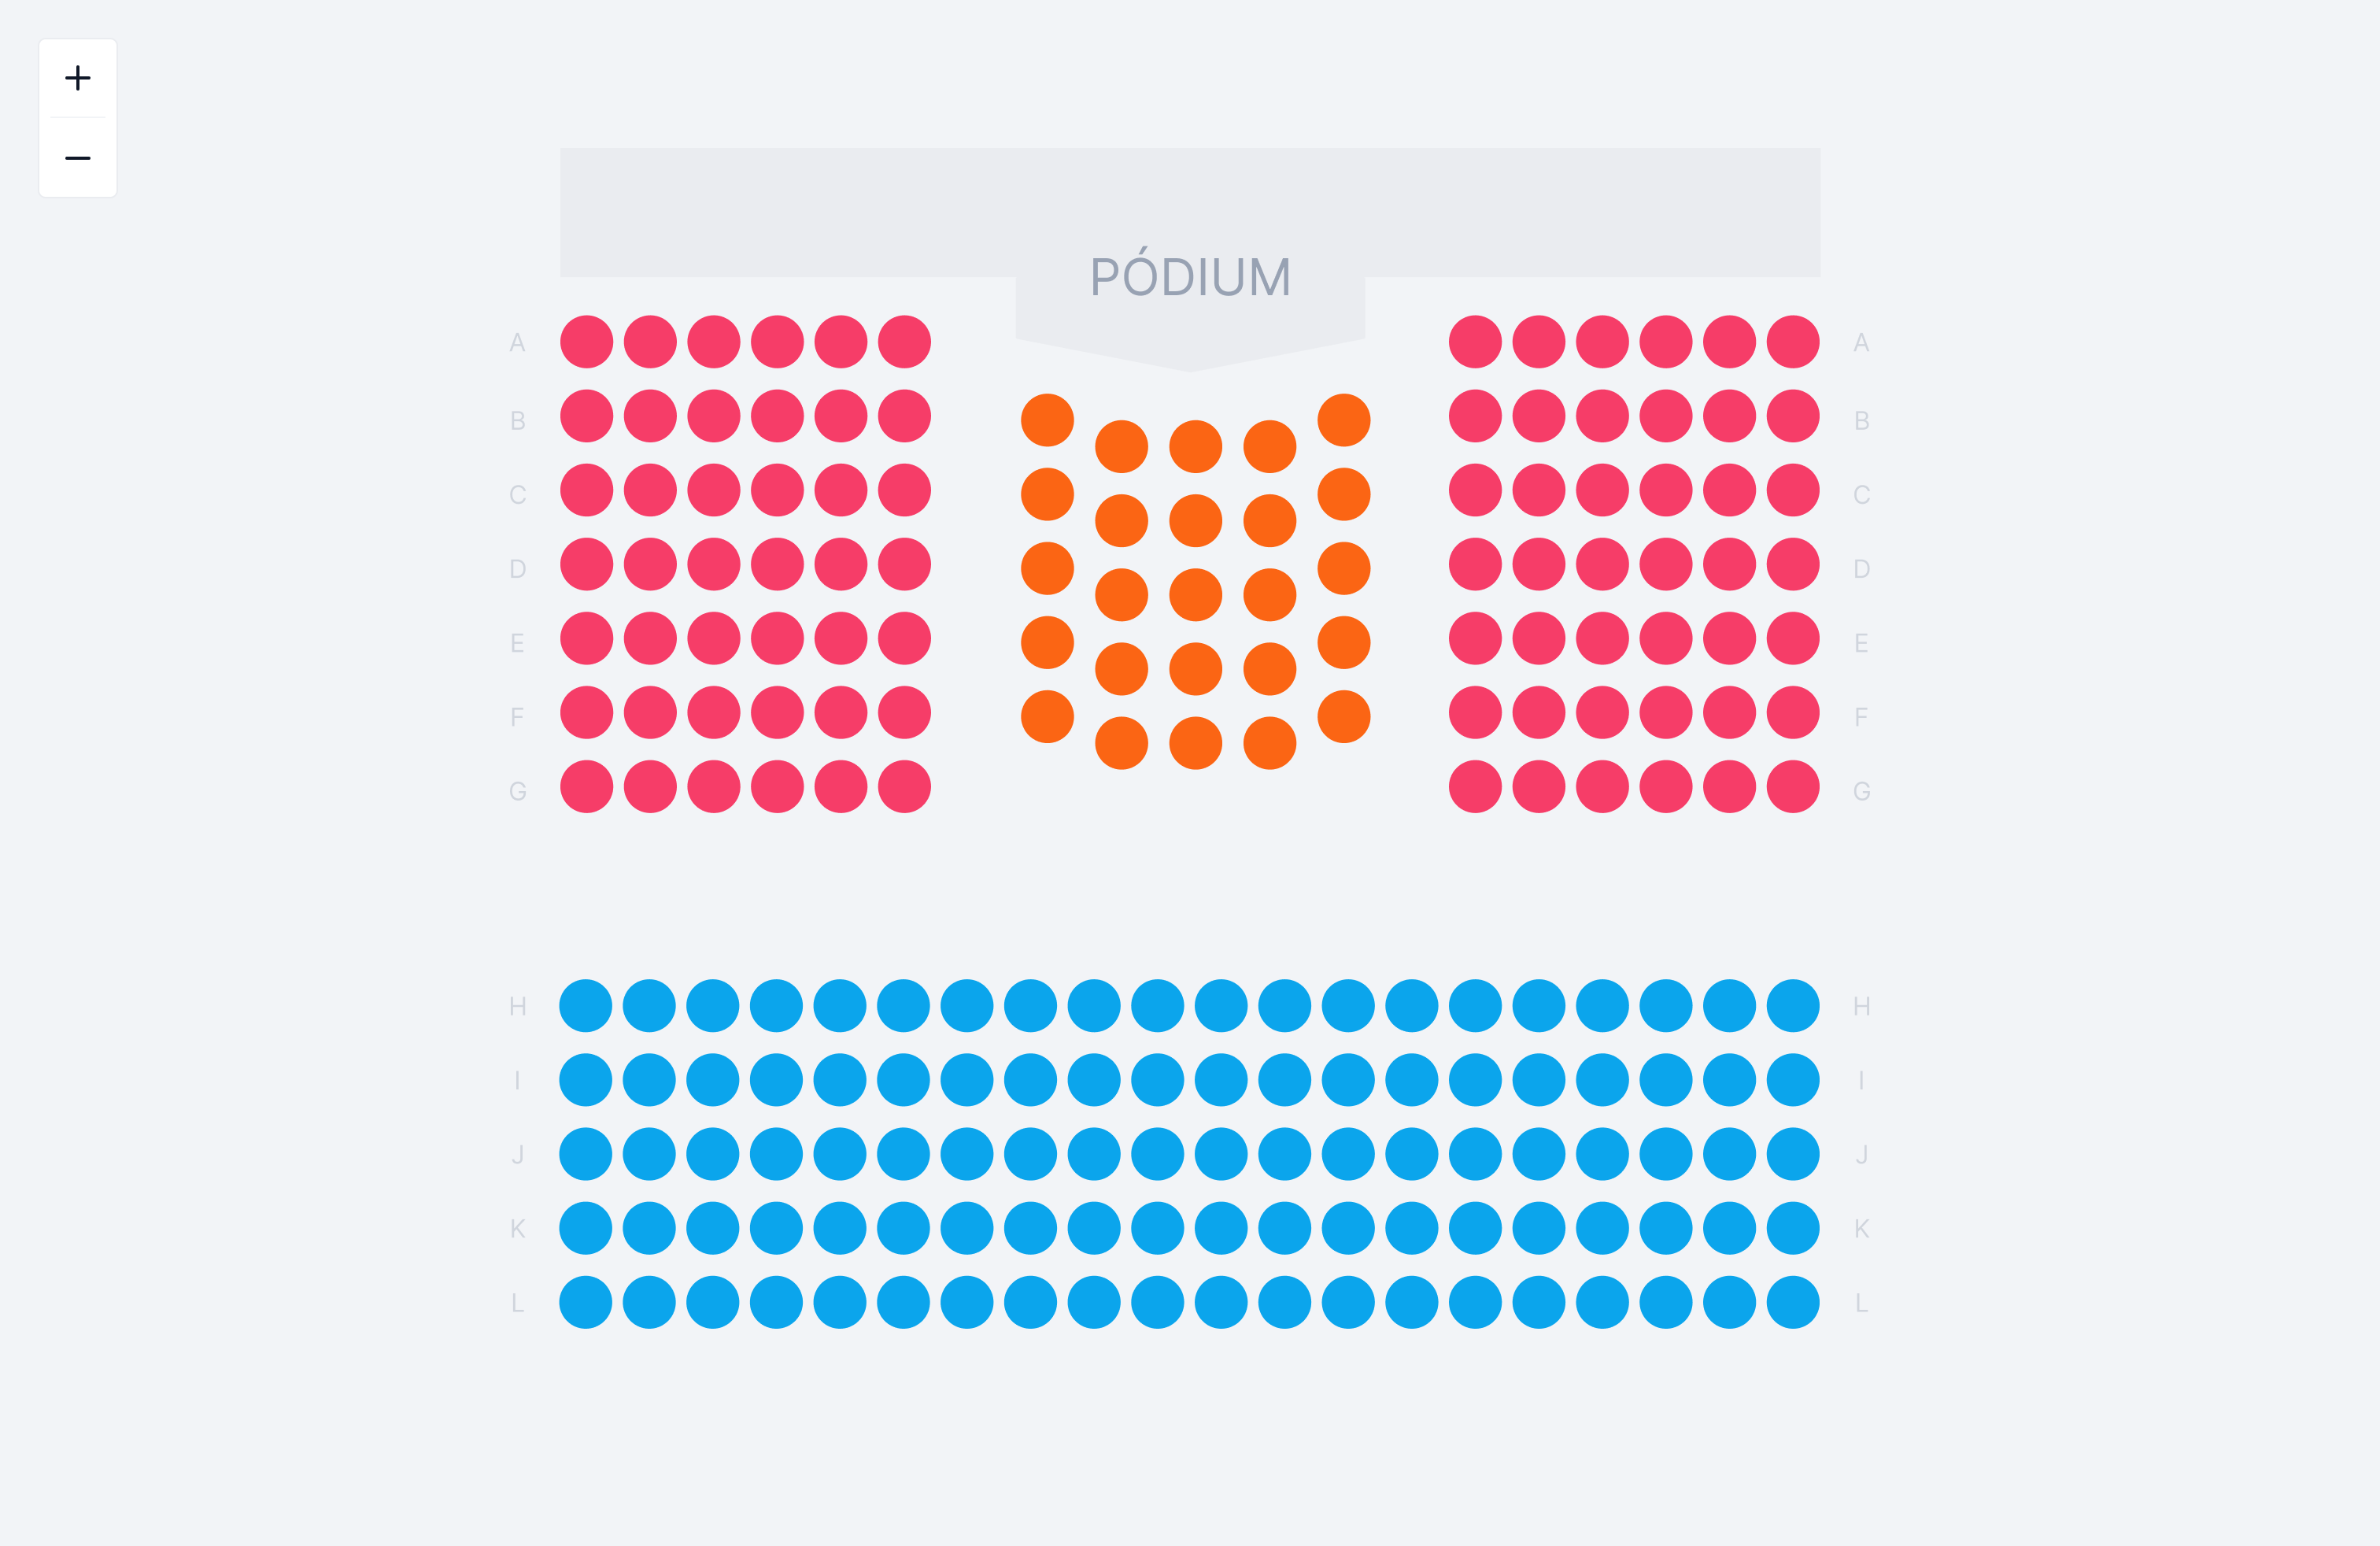
\includegraphics[width=\textwidth]{\FIGDIR/ui/us1-seating-map-desktop-1}
            \label{fig:us1-seating-map-desktop-1}
        \end{subfigure}
        \begin{subfigure}{0.2\textwidth}
            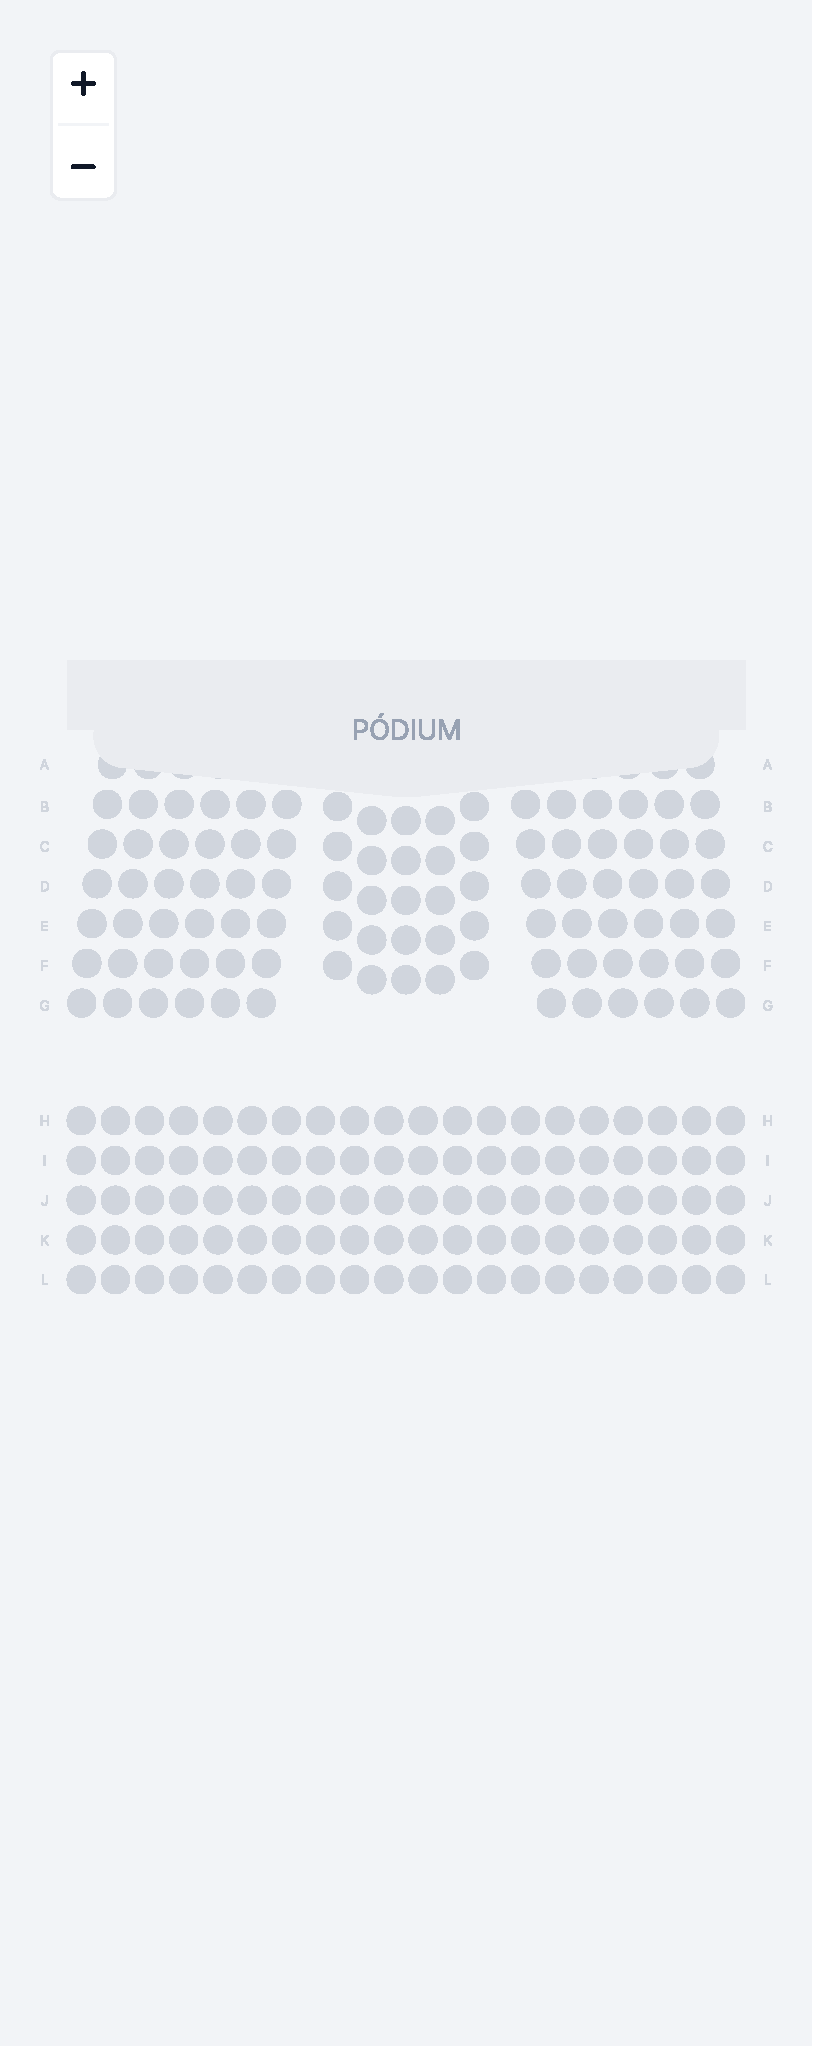
\includegraphics[width=\textwidth]{\FIGDIR/ui/us1-seating-map-mobile-1}
            \label{fig:us1-seating-map-mobile-1}
        \end{subfigure}
        \caption{Návrh komponent pro vizualizaci plánu sedadel místa konání}
        \label{fig:us1-seating-map}
    \end{figure}

    Na obrázku~\ref{fig:us1-seating-map} je zobrazen návrh komponenty, která by měla být schopna zobrazit plán sedadel místa konání.
    Součástí této komponenty je i boční ovládací panel, které umožňuje manuální přiblížení či oddálení plánu sedadel.
    U této komponenty se předpokládá, že její následná ovladatelnost bude primárně zajištěna pomocí myši, případně pomocí gest na dotykové obrazovce.

\end{subsection}

%%% Podsekce - Výběr sedadel
%%%%% Wording: ✅
%%%%% Styling: ✅
%%%%% References: ✅
%%%%% Grammar: ✅
%%% --------------------------------------------------------------
\begin{subsection}{Výběr sedadel}
    \label{subsec:narvh-ui-transformace-uzivatelskych-pribehu-vyber-sedadel}
    \userstoryseatselection

    Tento uživatelský příběh se zaměřuje na možnost výběru sedadel, která uživatelé chtějí zakoupit.
    Uživatelé by měli mít kontrolu nad výběrem svých sedadel, což implikuje potřebu rozhraní, které nejen zobrazuje plán sedadel, ale také umožňuje interaktivní výběr a zrušení výběru jednotlivých sedadel.

    Praktickým řešením tohoto uživatelského příběhu může být přidání klikacích prvků do plánu sedadel, které budou reprezentovat jednotlivá sedadla.
    Tyto prvky by měly po interakci jasně indikovat stav výběru či zrušení výběru, poskytující uživateli okamžitou vizuální zpětnou vazbu.

    Jakmile je sedadlo vybráno, plán sedadel by měl tuto volbu odrazit změnou barvy sedadla nebo přidáním výrazného značení.
    Stejně tak, pokud je sedadlo zrušeno, mělo by se vrátit do svého původního stavu.
    Tato vizuální zpětná vazba nejen potvrzuje akci uživatele, ale také jim pomáhá sledovat jejich výběry, když se pohybují po místě konání.

    V otázce funkčnosti, je zásadní zajistit, aby proces výběru a zrušení výběru byl intuitivní a bezchybný.
    Pokud je sedadlo již zarezervováno či z jiného důvodu nedostupné, uživatelské rozhraní by mělo zabránit jeho výběru.

    \begin{figure}[H]
        \centering
        \begin{subfigure}{0.775\textwidth}
            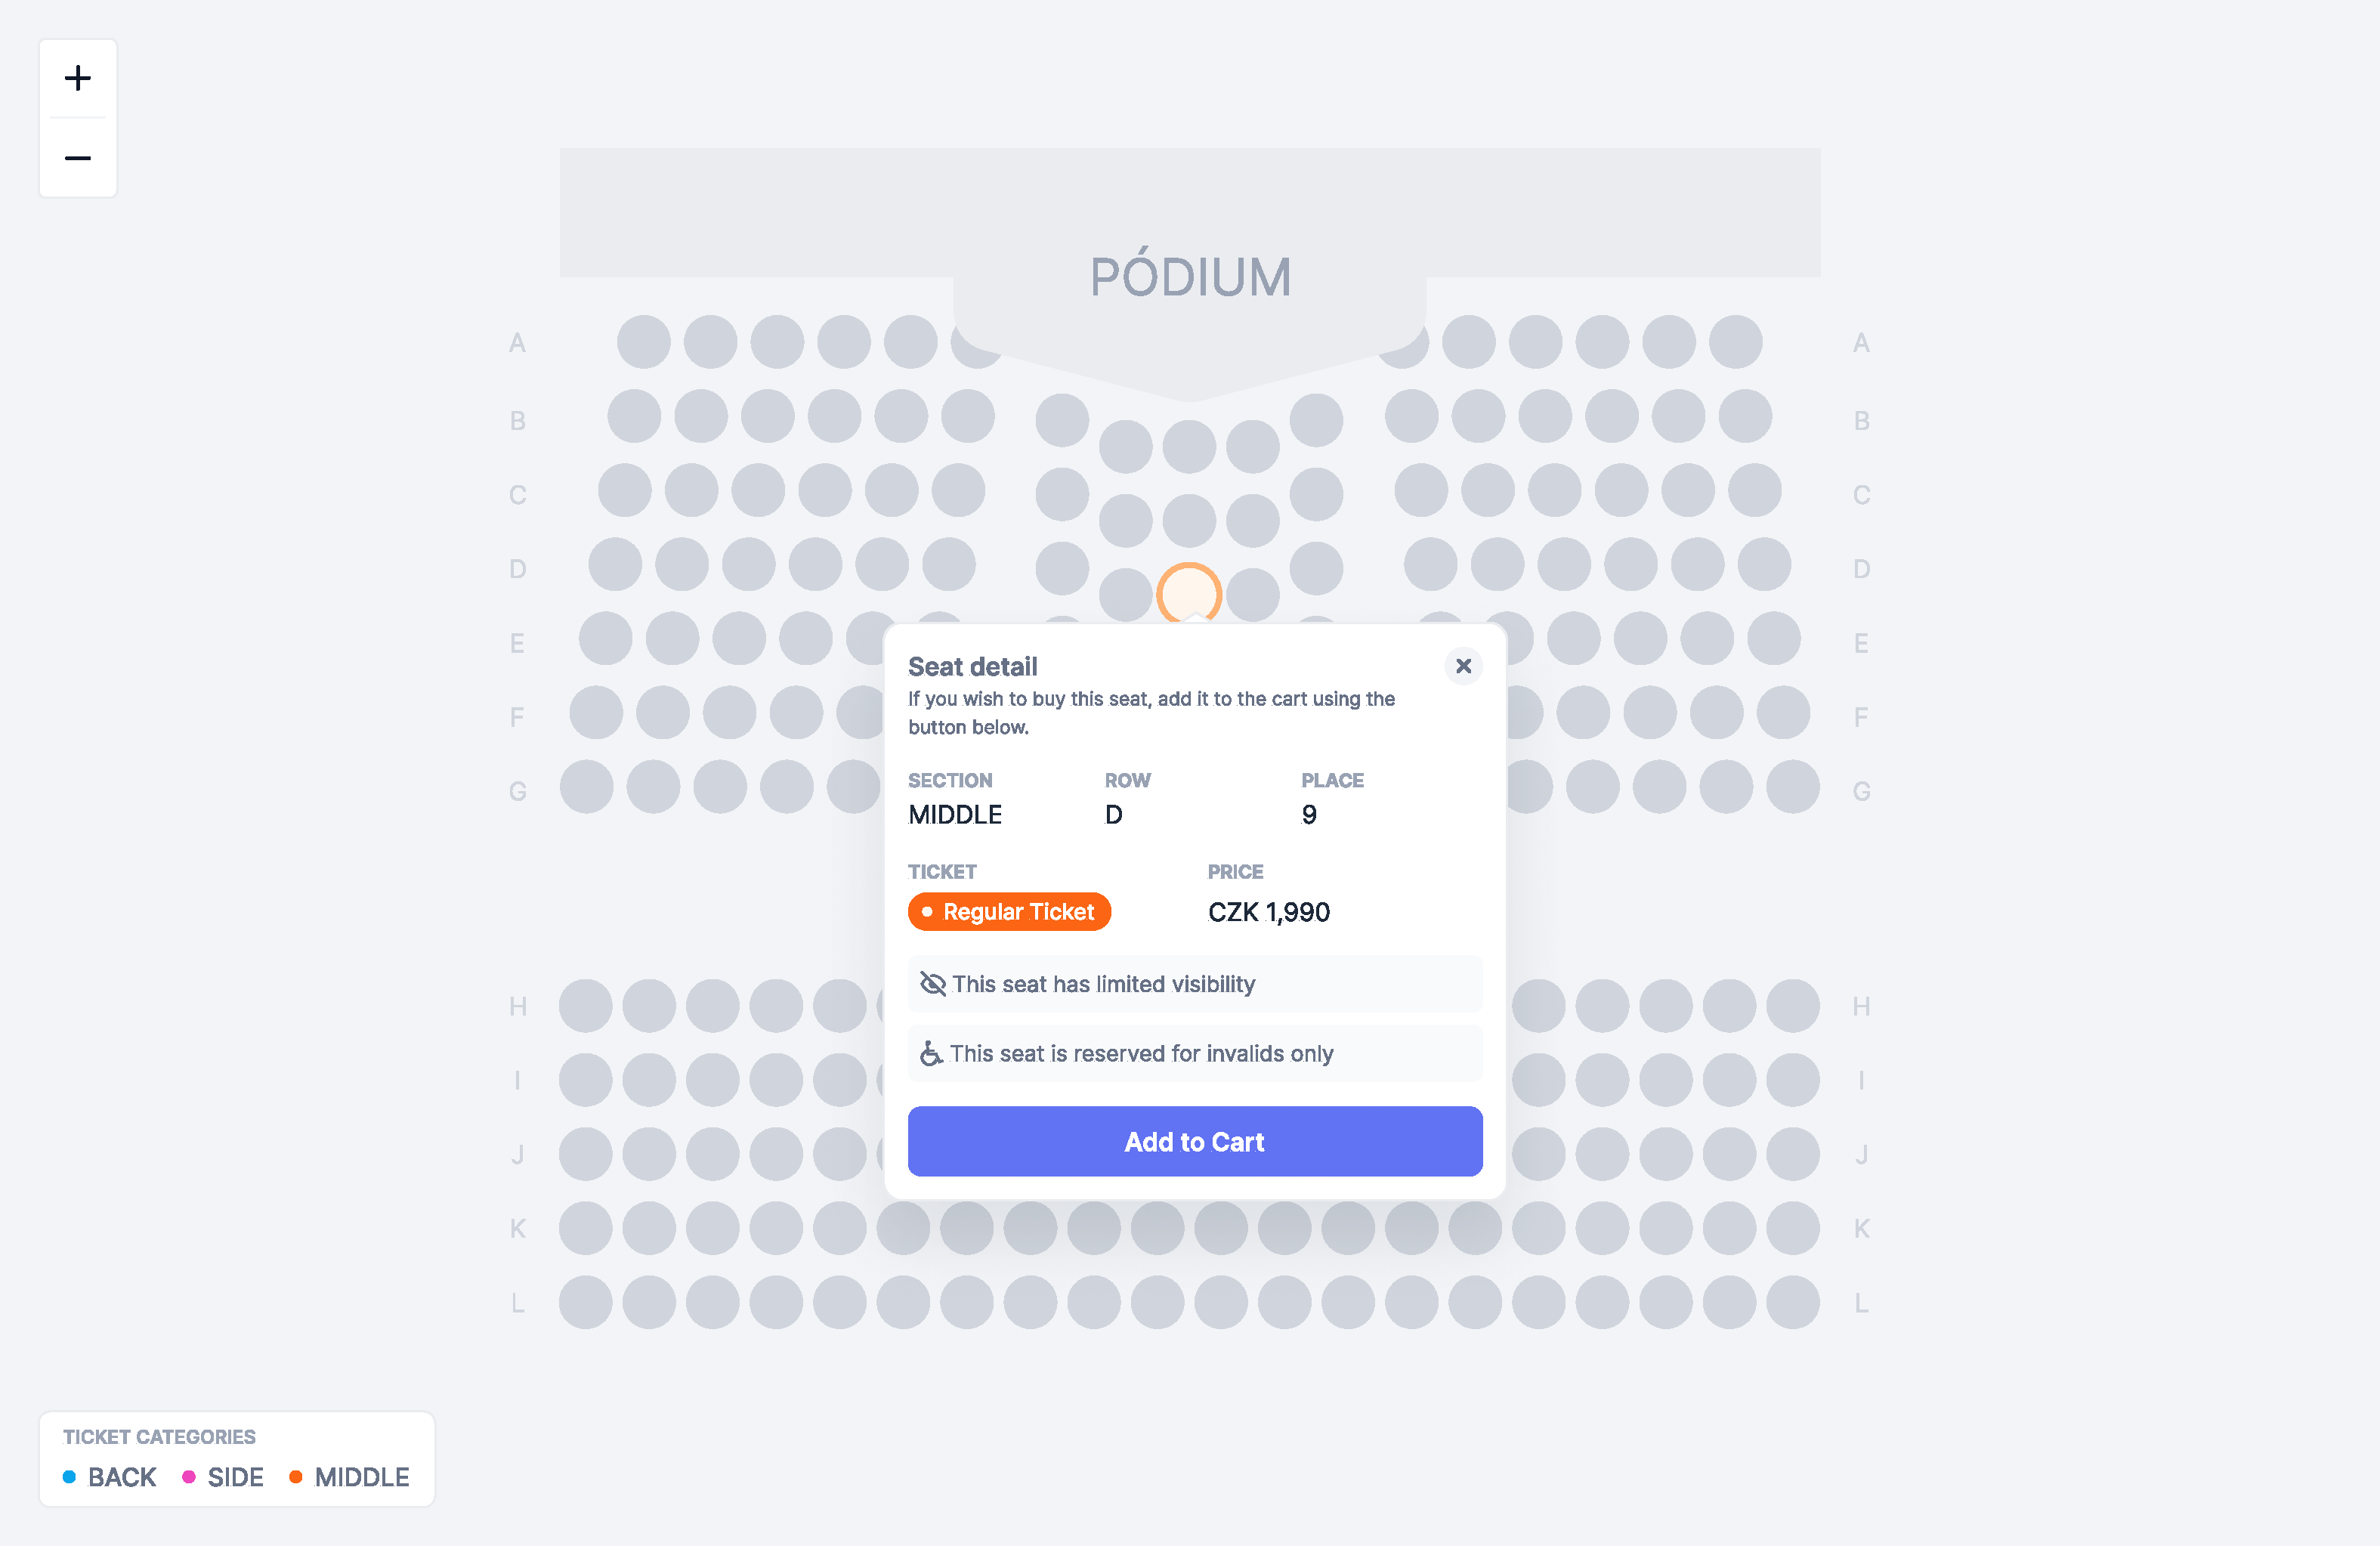
\includegraphics[width=\textwidth]{\FIGDIR/ui/us2-seat-selection-desktop-1}
            \label{fig:us2-seat-selection-desktop-1}x
        \end{subfigure}
        \begin{subfigure}{0.2\textwidth}
            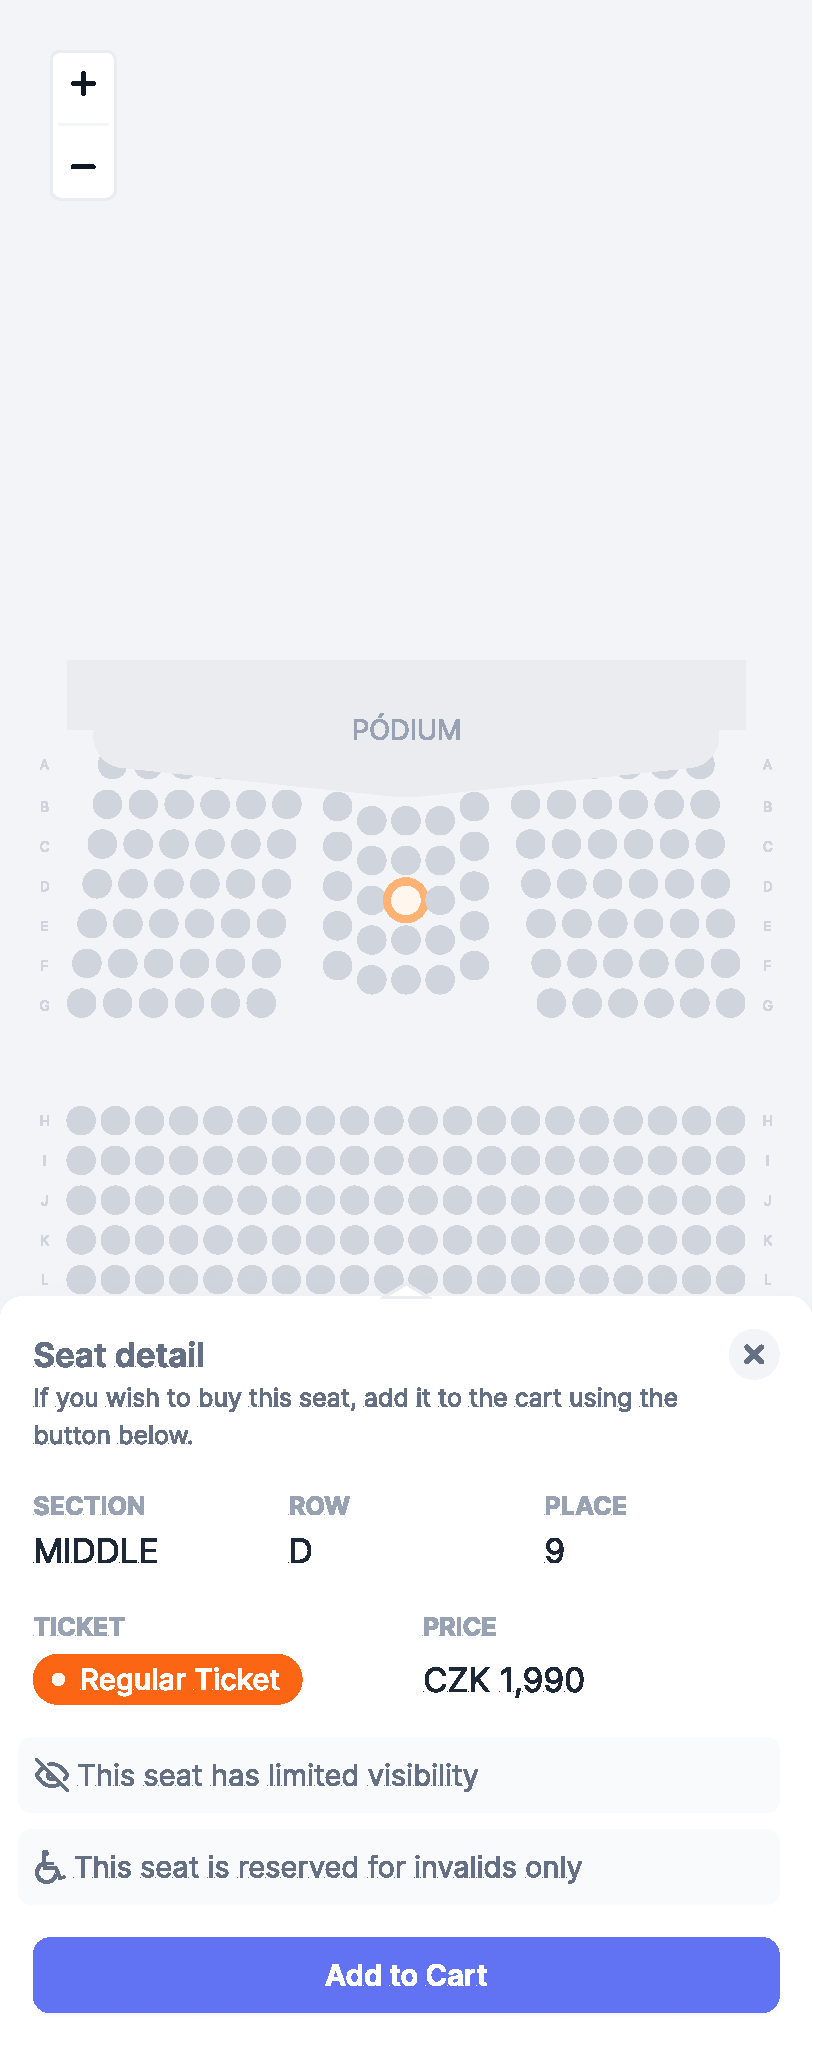
\includegraphics[width=\textwidth]{\FIGDIR/ui/us2-seat-selection-mobile-1}
            \label{fig:us2-seat-selection-mobile-1}
        \end{subfigure}
        \caption{Návrh komponent pro výběr sedadel}
        \label{fig:us2-seat-selection}
    \end{figure}

    Na obrázku~\ref{fig:us2-seat-selection} je vyobrazen návrh interaktivní komponenty plánu míst, která umožňuje výběr sedadel.
    Volná sedadla k výběru jsou označena výraznými barvami, které odpovídají jejím cenovým kategoriím.
    Tyto kategorie, pro větší přehlednost, jsou zobrazeny v legendě, která je umístěna v pravém dolním rohu komponenty.

    Pro tuto komponentu je zásadní jasně rozpoznat různé stavy sedadel, jako například dostupné, nedostupné, již přidané či aktuálně označené.
    Některé tyto stav mohou být navíc i různě kombinovány, jako například již přidané a aktuálně označené sedadlo.
    Tyto stavy jsou zobrazeny v rámci návrhy komponenty \foreign{Seat} na obrázku~\ref{fig:component-seat} níže.

    \begin{figure}[H]
        \centering
        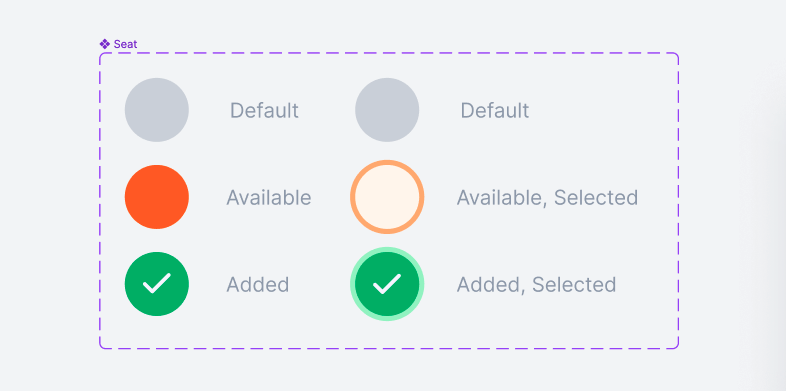
\includegraphics[width=\textwidth]{\FIGDIR/ui/component-seat}
        \caption{Komponenta sedadla a její stavy}
        \label{fig:component-seat}
    \end{figure}

    Součástí návrh této komplexní komponenty, ačkoliv není přímo součástí uživatelského příběhu, je i komponenta zobrazující přehledný detail právě vybraného sedadla.
    Sedadla totiž mohou nést různé informace, jako například číslo sedadla, jeho kategorie, cena, či informace o tom, zda je již obsazené nebo má například zhoršenou viditelnost na jeviště.
    Hlavní funkcí této komponenty je potvrzení výběru sedadla, tedy jeho přidání do košíku, či zrušení výběru.
    Na obrázku~\ref{fig:component-seat-} je vyobrazen návrh této komponenty.

    \begin{figure}[H]
        \centering
        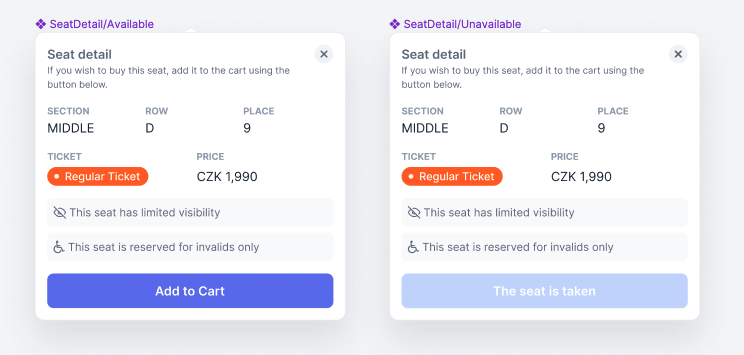
\includegraphics[width=\textwidth]{\FIGDIR/ui/component-seat-detail}
        \caption{Komponenta detailu zvoleného sedadla}
        \label{fig:component-seat-}
    \end{figure}

    Tato komponenta funguje jakési modální okno, které se zobrazí po kliknutí na sedadlo.
    Ovšem jeho zobrazení je specifické na desktopové a mobilní verzi, jak je vyobrazeno na obrázku~\ref{fig:us2-seat-selection}.
    Na desktopové verzi se zobrazí jako popover okno umístěné u právě označeného sedadla.
    Na mobilní verzi se toto okno chová jako fixně umístěný list, který se zobrazí v dolní části obrazovky.
    Díky umístění v dolní části obrazovky na mobilních zařízeních se tak zajistí komfortní ovládání a interakce s tímto listem, jelikož se nachází v dosahu palce neboli v tzv. \foreign{thumb zone}.
\end{subsection}

%%% Podsekce - Nákupní košík
%%%%% Wording: ✅
%%%%% Styling: ✅
%%%%% References: ✅
%%%%% Grammar: ✅
%%% --------------------------------------------------------------
\begin{subsection}{Nákupní košík}
    \label{subsec:narvh-ui-transformace-uzivatelskych-pribehu-nakupni-kosik}
    \userstoryshoppingcart

    Uživatel se nyní již umí pohybovat na mapě místa konání a vybrat si sedadlo, které chce zakoupit.
    Tento uživatelský příběh poukazuje na nutnost jasného přehledu aktuálního stavu nákupního košíku.
    Nákupní košík by měl uživateli sloužit jako přehled přidaných vstupenek s dalšími informacemi, jako například cena, kategorie, či počet vstupenek.
    Nákupní košík by také měl zobrazovat celkovou cenu všech vstupenek, které jsou v něm obsaženy.
    Poskytnutím těchto informací může zákazník potvrdit svůj výběr, sledovat celkovou cenu objednávky a rozhodnout se, zda bude pokračovat v nákupu, či provede úpravy.

    Ačkoliv není v uživatelském příběhu nijak definováno, lze z technických požadavků předpokládat, že celý proces vytváření objednávky bude probíhat v rámci rezervace pro zajištění zaručeného výběru sedadel.
    Tato rezervace bude mít časový limit, po jehož vypršení bude rezervace automaticky zrušena a sedadla budou opět uvolněna k prodeji.
    Tuto informaci je tedy taktéž nezbytné zobrazit ideálně v rámci této komponenty nákupního košíku.
    Tuto komponentu nákupního košíku lze také použít jako navigační prvek, který umožní uživateli přejít k dalším krokům v procesu nákupu.

    Na obrázku~\ref{fig:us3-cart-summary-desktop} je vyobrazen návrh komponenty přehledu nákupního košíku v desktopové verzi.
    Díky velkému prostoru, který je na desktopových zařízených k dispozici, je možné zobrazit všechny informace o vstupenkách, které jsou v košíku obsaženy.
    Tuto komponentu lze vyobrazit jako postranní panel, obsahující všechny tyto informace.
    Díky umístění této komponenty na pravou strany celé obrazovky, kterou pokrývá komponenta mapy sedadel, je zajištěno, že uživatel bude mít vždy přehled o svém výběru, bude jasně viditelný a vyplní zbytečně nevyužitý prostor na obrazovce.

    \begin{figure}[H]
        \centering
        \begin{subfigure}{\textwidth}
            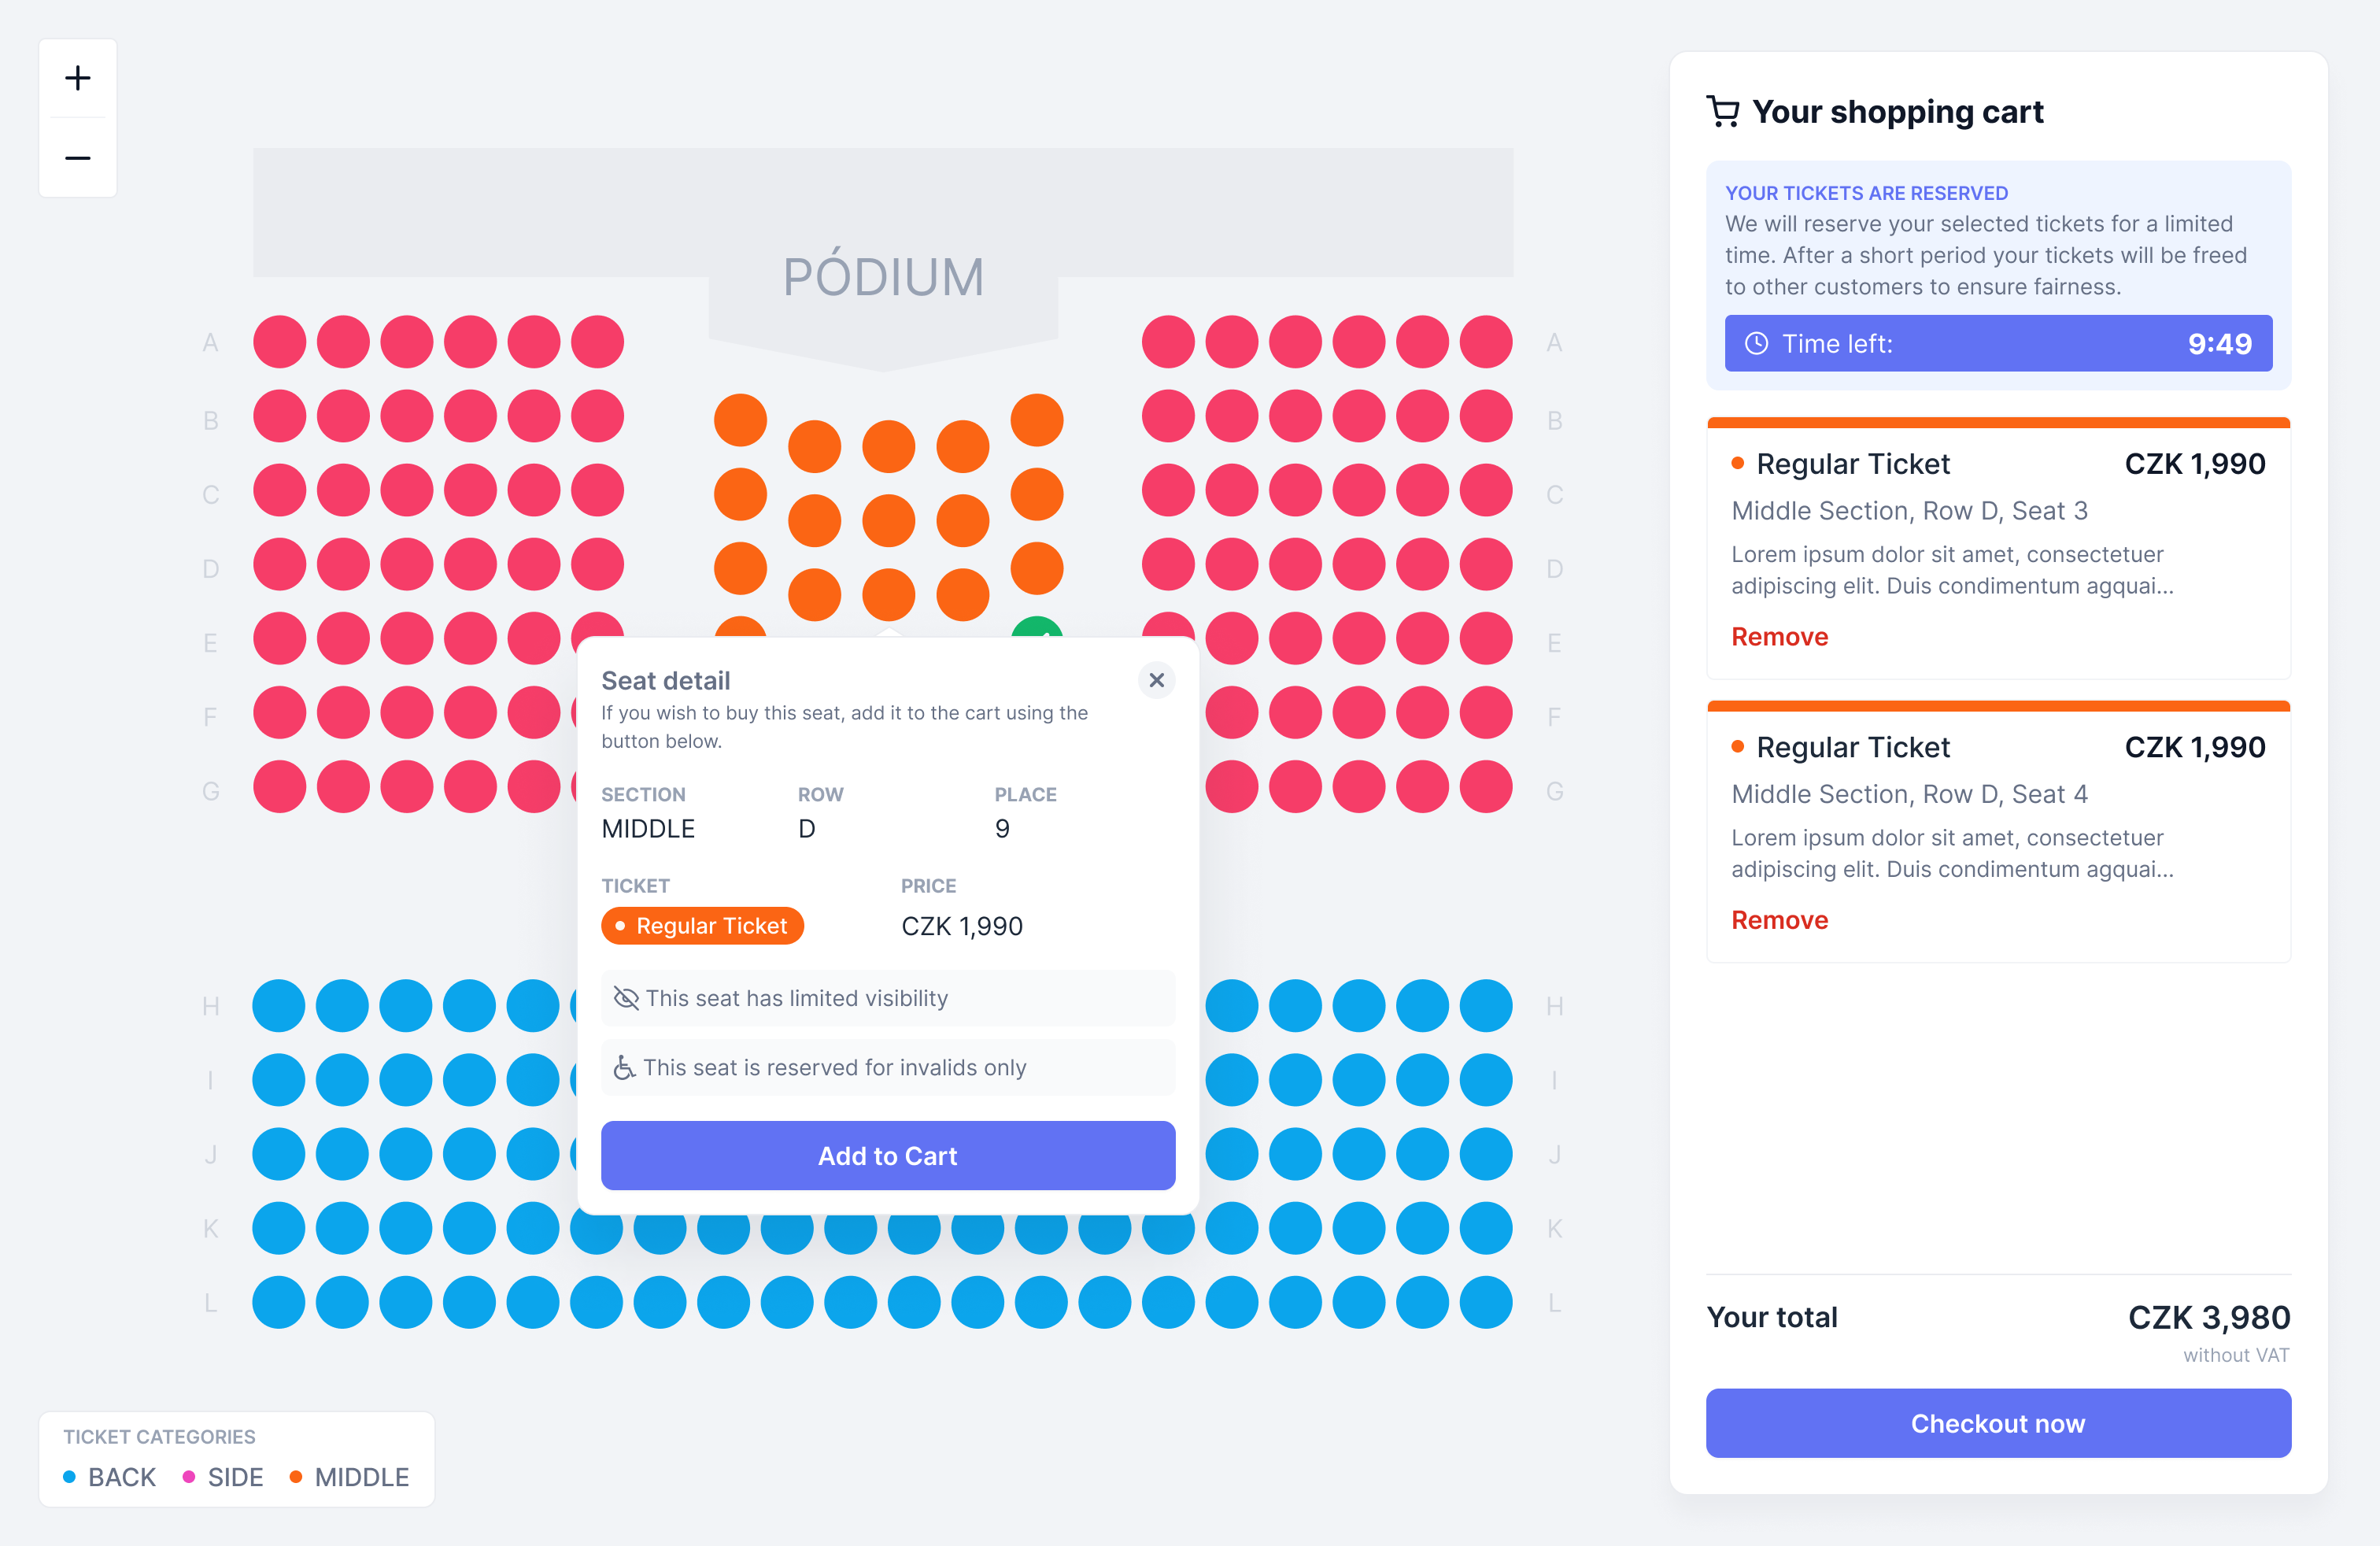
\includegraphics[width=\textwidth]{\FIGDIR/ui/us3-cart-summary-desktop-1}
            \label{fig:uus3-cart-summary-desktop-1}
        \end{subfigure}
        \caption{Návrh komponent přehledu nákupního košíku (desktopová verze)}
        \label{fig:us3-cart-summary-desktop}
    \end{figure}

    Na mobilní verzi je situace poněkud odlišná.
    V této situaci je k dispozici mnohem méně prostoru, a proto je nutné zobrazit pouze nejdůležitější informace.
    Sekundární informace, jako například cena, či kategorie vstupenky, lze zobrazit například až po rozbalení detailu nákupního košíku.

    \begin{figure}[H]
        \centering
        \begin{subfigure}{0.4\textwidth}
            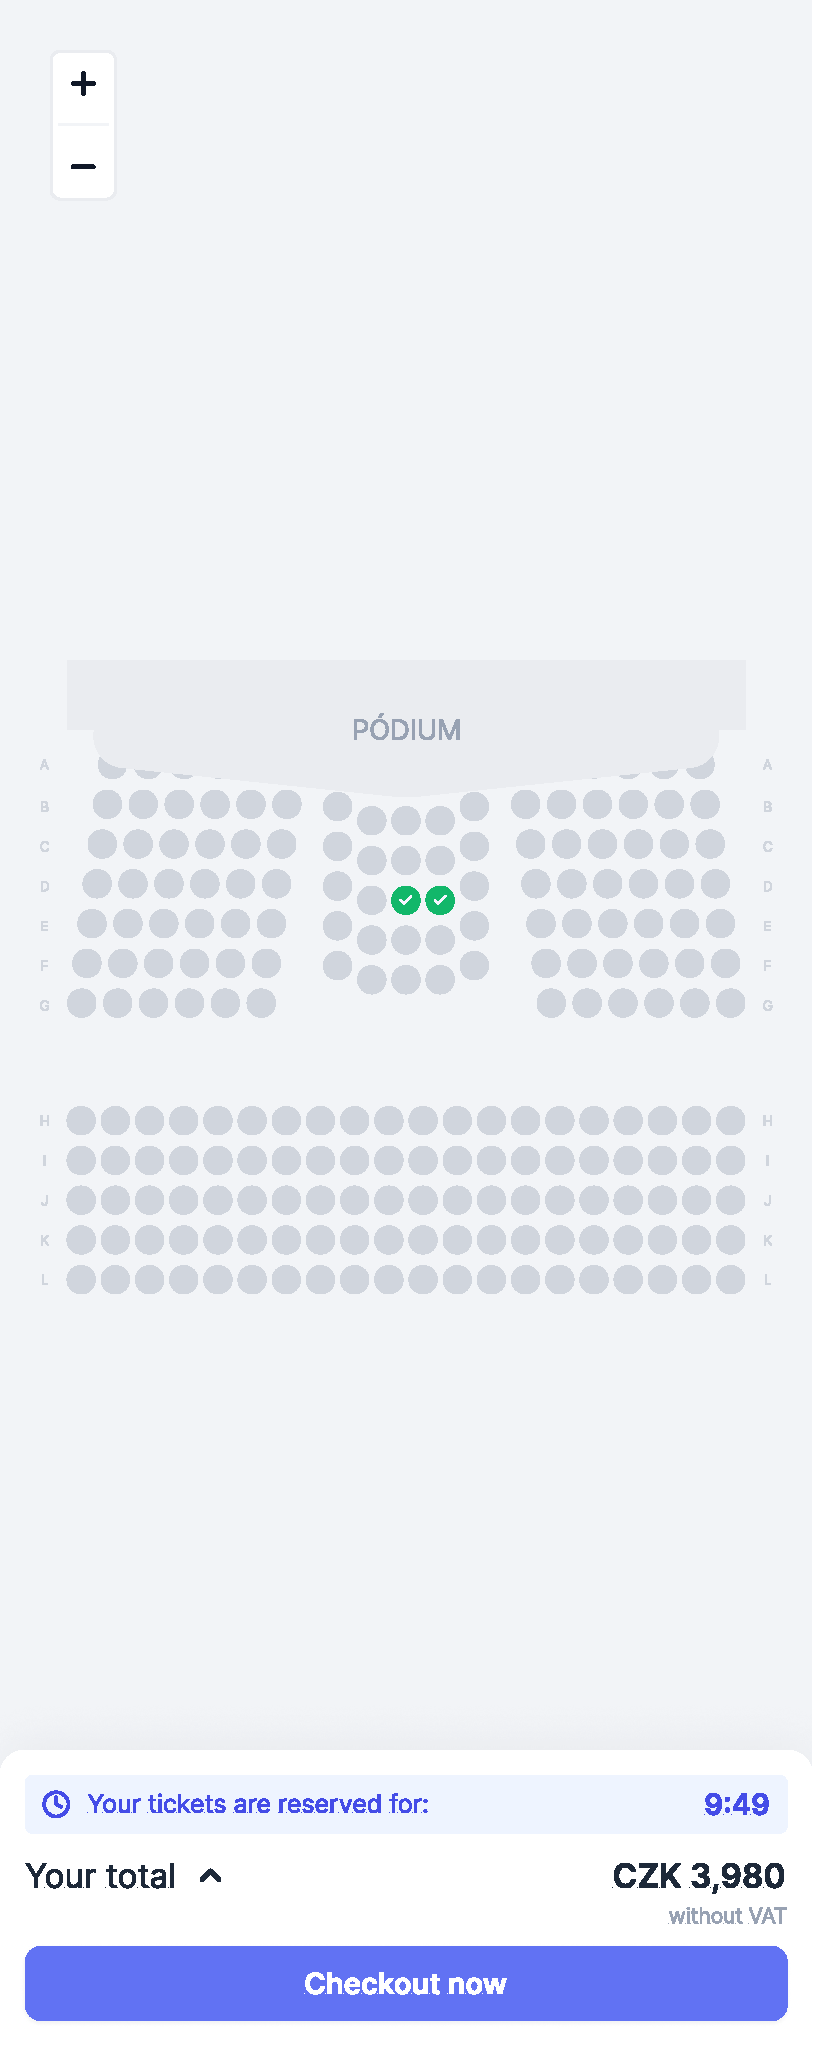
\includegraphics[width=\textwidth]{\FIGDIR/ui/us3-cart-summary-mobile-1}
            \caption{sbaleno}
            \label{fig:us3-cart-summary-mobile-1}
        \end{subfigure}
        \hfill
        \begin{subfigure}{0.4\textwidth}
            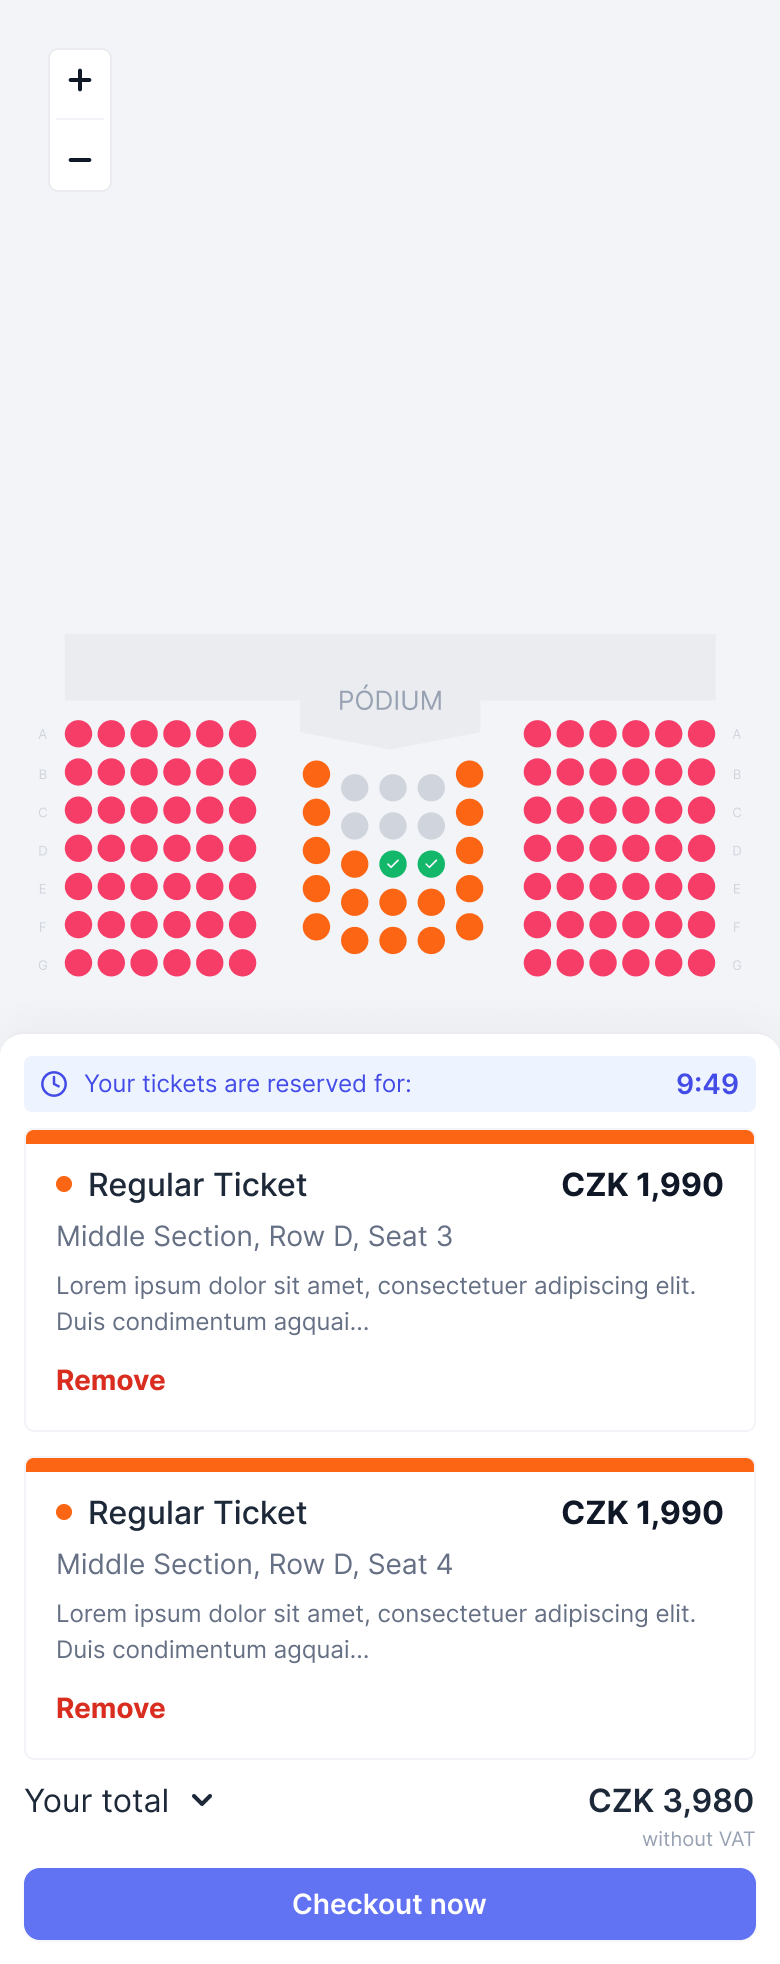
\includegraphics[width=\textwidth]{\FIGDIR/ui/us3-cart-summary-mobile-2}
            \caption{rozbaleno}
            \label{fig:us3-cart-summary-mobile-2}
        \end{subfigure}

        \caption{Návrh komponent přehledu nákupního košíku (mobilní verze)}
        \label{fig:us3-cart-summary-mobile}
    \end{figure}

    Na obrázku~\ref{fig:us3-cart-summary-mobile} je návrh komponenty přehledu nákupního košíku v mobilní verzi, která je umístěna v dolní části obrazovky, aby byla v dosahu palce, a zároveň nezakrývala žádnou důležitou informaci.
    Ve výchozím (sbaleném) stavu obsahuje pouze ty nejdůležitější informace, jako celkovou cenu objednávky.
    Po rozbalení detailu nákupního košíku se zobrazí všechny informace o vstupenkách, které jsou v košíku obsaženy, podobně jako je tomu v desktopové verzi.
\end{subsection}

%%% Podsekce - Vyřízení a potvrzení objednávky
%%%%% Wording: ✅
%%%%% Styling: ✅
%%%%% References: ✅
%%%%% Grammar: ✅
%%% --------------------------------------------------------------
\begin{subsection}{Vyřízení a potvrzení objednávky}
    \label{subsec:narvh-ui-transformace-uzivatelskych-pribehu-vyrideni-a-potvrzeni-objednavky}
    \userstorycheckout

    Proces vyřízení objednávky je posledním krokem v procesu nákupu vstupenek (pokud pomineme krok placení, který není řešen v rámci této práce).
    V tomto kroku je uživatel vyzván k zadání svých osobních údajů, které jsou nutné pro dokončení objednávky.
    Tyto údaje, pro jednoduchost, zahrnují pouze jméno, příjmení, e-mailovou adresu a telefonní kontakt.
    V reálném nasazení by bylo vhodné zahrnout i další údaje, jako například fakturační adresu, či případně další kontaktní údaje.
    Jako speciální údaj lze zákazníkovi nabídnout i možnost vyplnění poznámky k objednávce, která by mohla obsahovat například požadavek na zaslání faktury, či jiné informace.

    Návrh celé této komplexní komponenty je zobrazen na obrázku~\ref{fig:us4-cart-checkout-desktop} níže.
    Tato komponenta, jak je zřejmé, je složena z několika dalších menších částí.

    \begin{figure}[H]
        \centering
        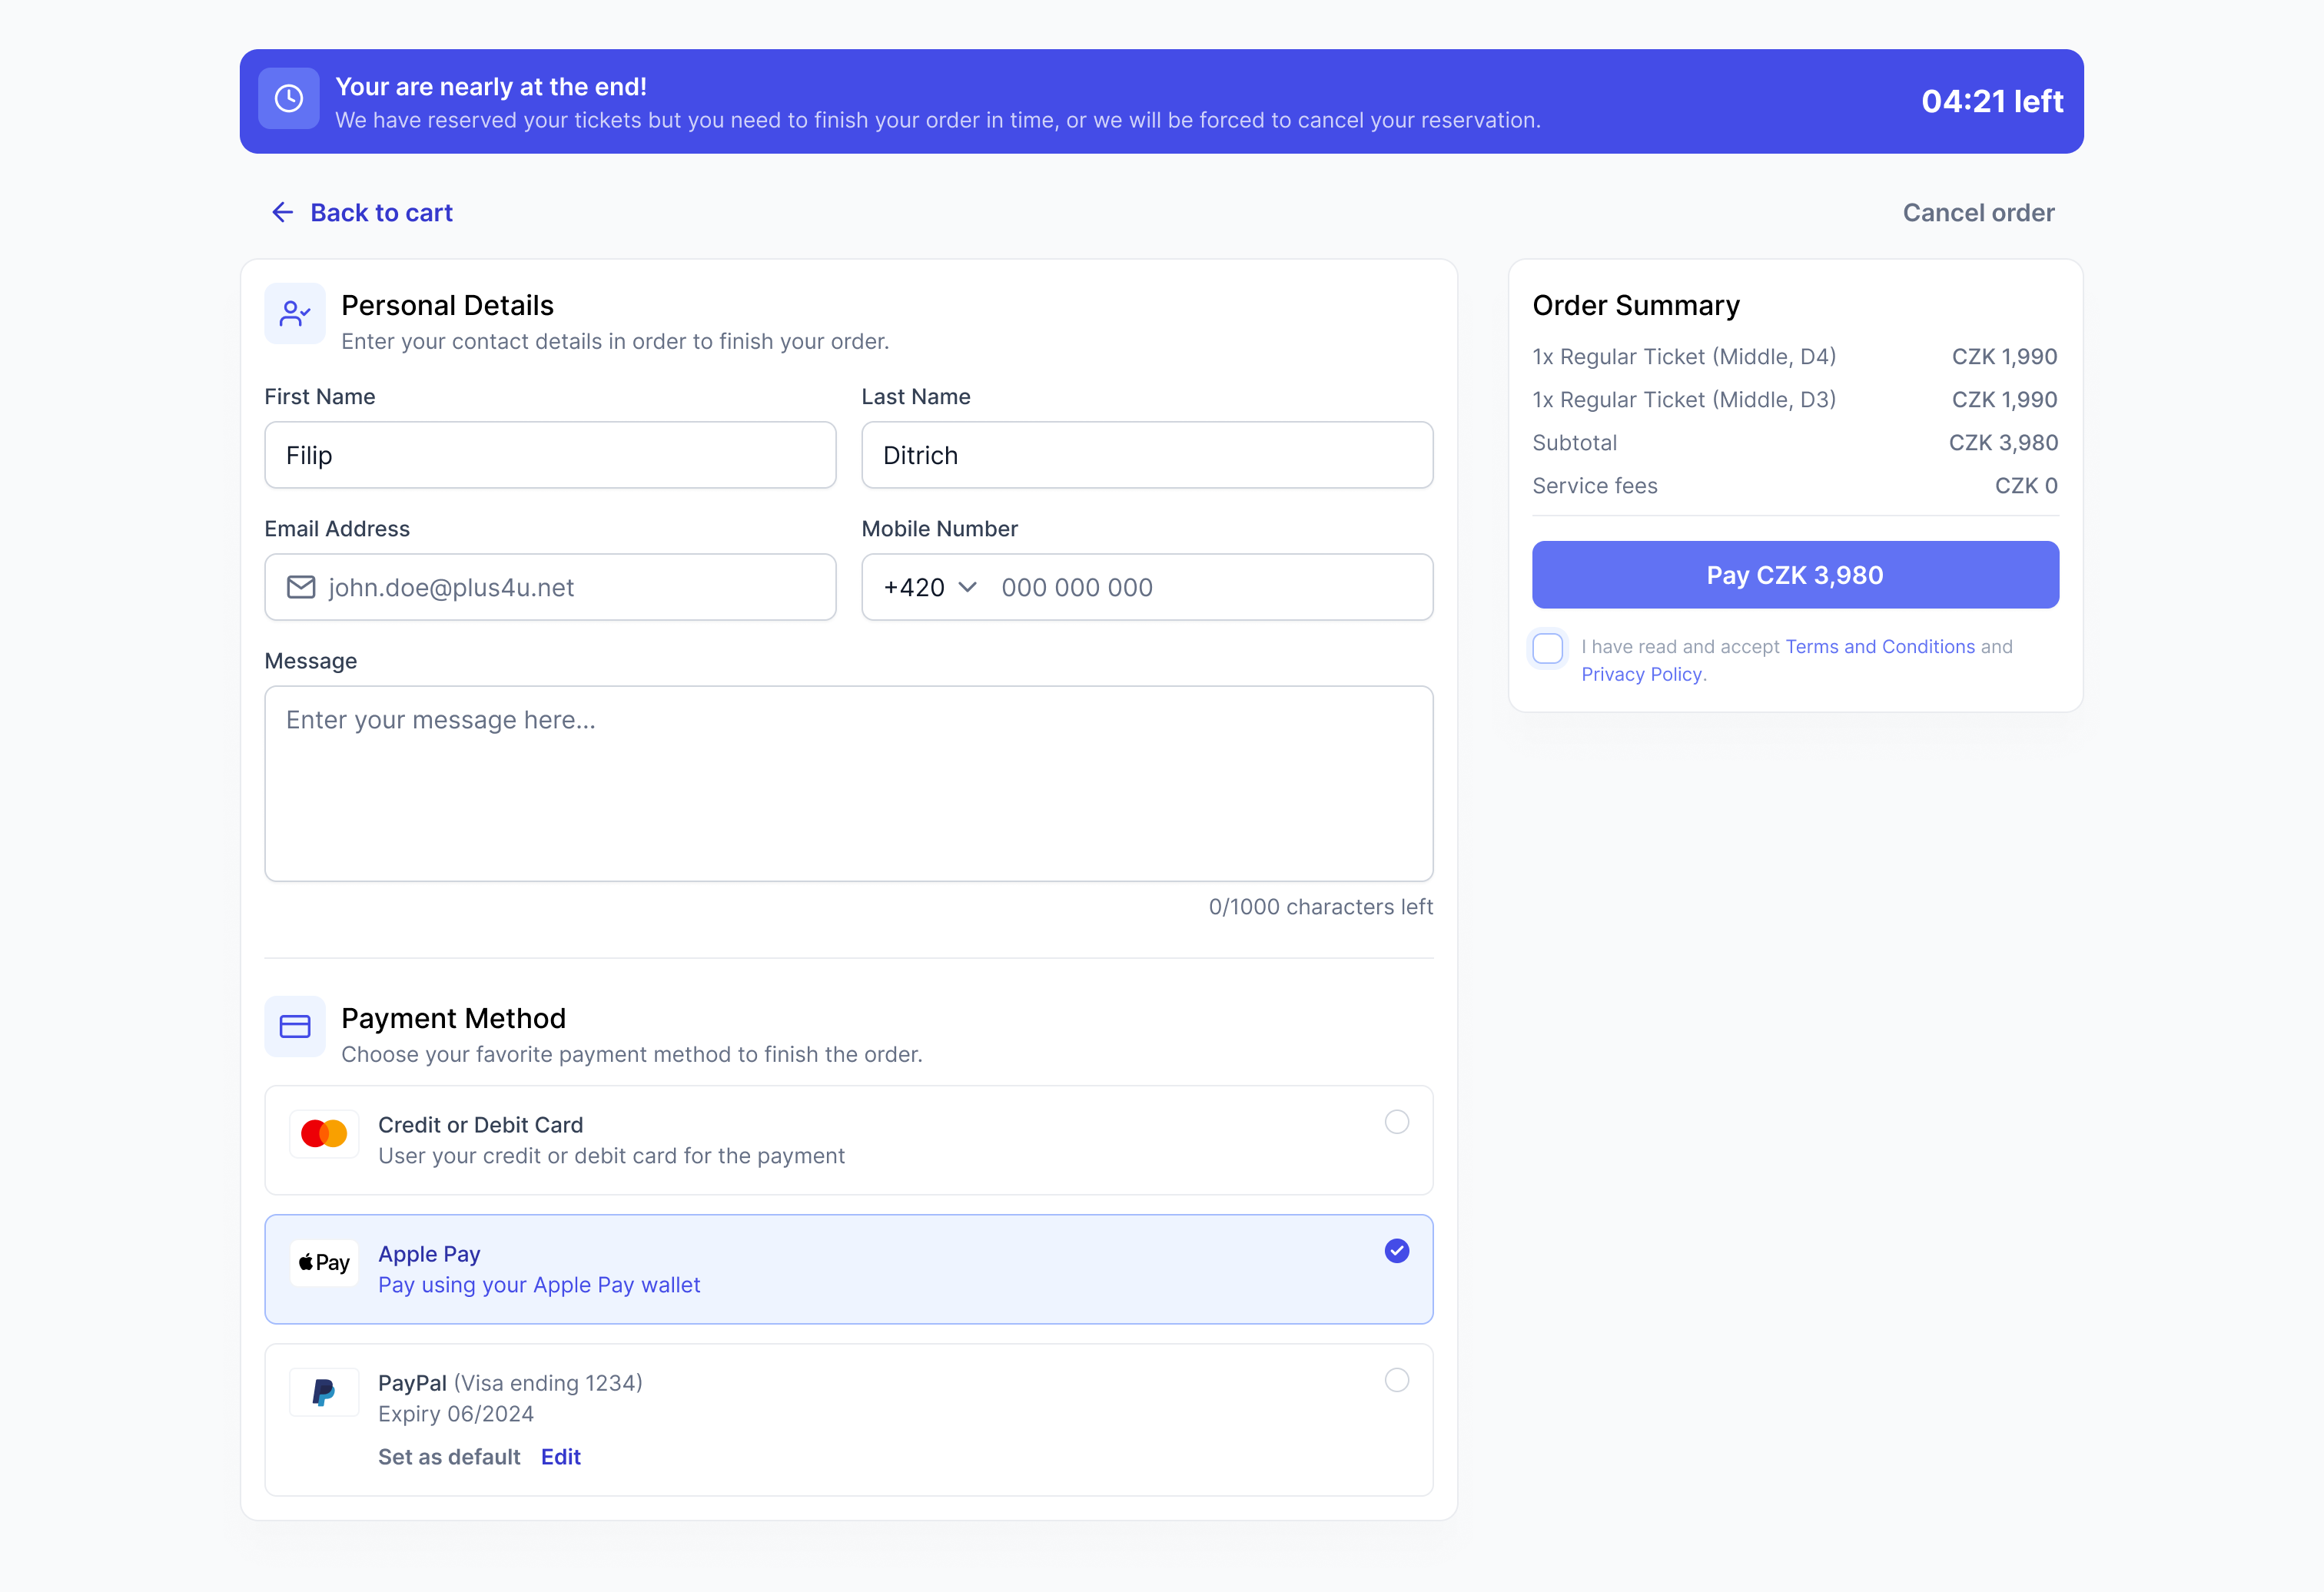
\includegraphics[width=\textwidth]{\FIGDIR/ui/us4-cart-checkout-desktop-1}
        \caption{Návrh komponent dokončení objednávky (desktopová verze)}
        \label{fig:us4-cart-checkout-desktop}
    \end{figure}

    Primární částí je formulář, který obsahuje všechny potřebné údaje pro dokončení objednávky.
    Následuje výběr platební metody a souhrn objednávky, aby měl zákazník stálý přehled o jeho objednávce.
    V neposlední řádě je zde stále zobrazena informace o probíhající rezervaci objednávky a jejím časovém limitu, v rámci, kterého musí zákazník objednávku dokončit, jinak bude rezervace zrušena.
    Dále je zákazníkovi umožněno přejít zpět do procesu výběru vstupenek pomocí tlačítka \foreign{Back to cart} či proces vytváření objednávky kompletně zrušit pomocí tlačítka \foreign{Cancel order}.

    V mobilním rozlišení je zobrazení této komponenty pouze mírně upraveno zarovnáním a umístěním všech prvků do jednoho sloupce, jak je zobrazeno na obrázku~\ref{fig:us4-cart-checkout-mobile} níže.

    \begin{figure}[H]
        \centering
        \begin{subfigure}{0.4\textwidth}
            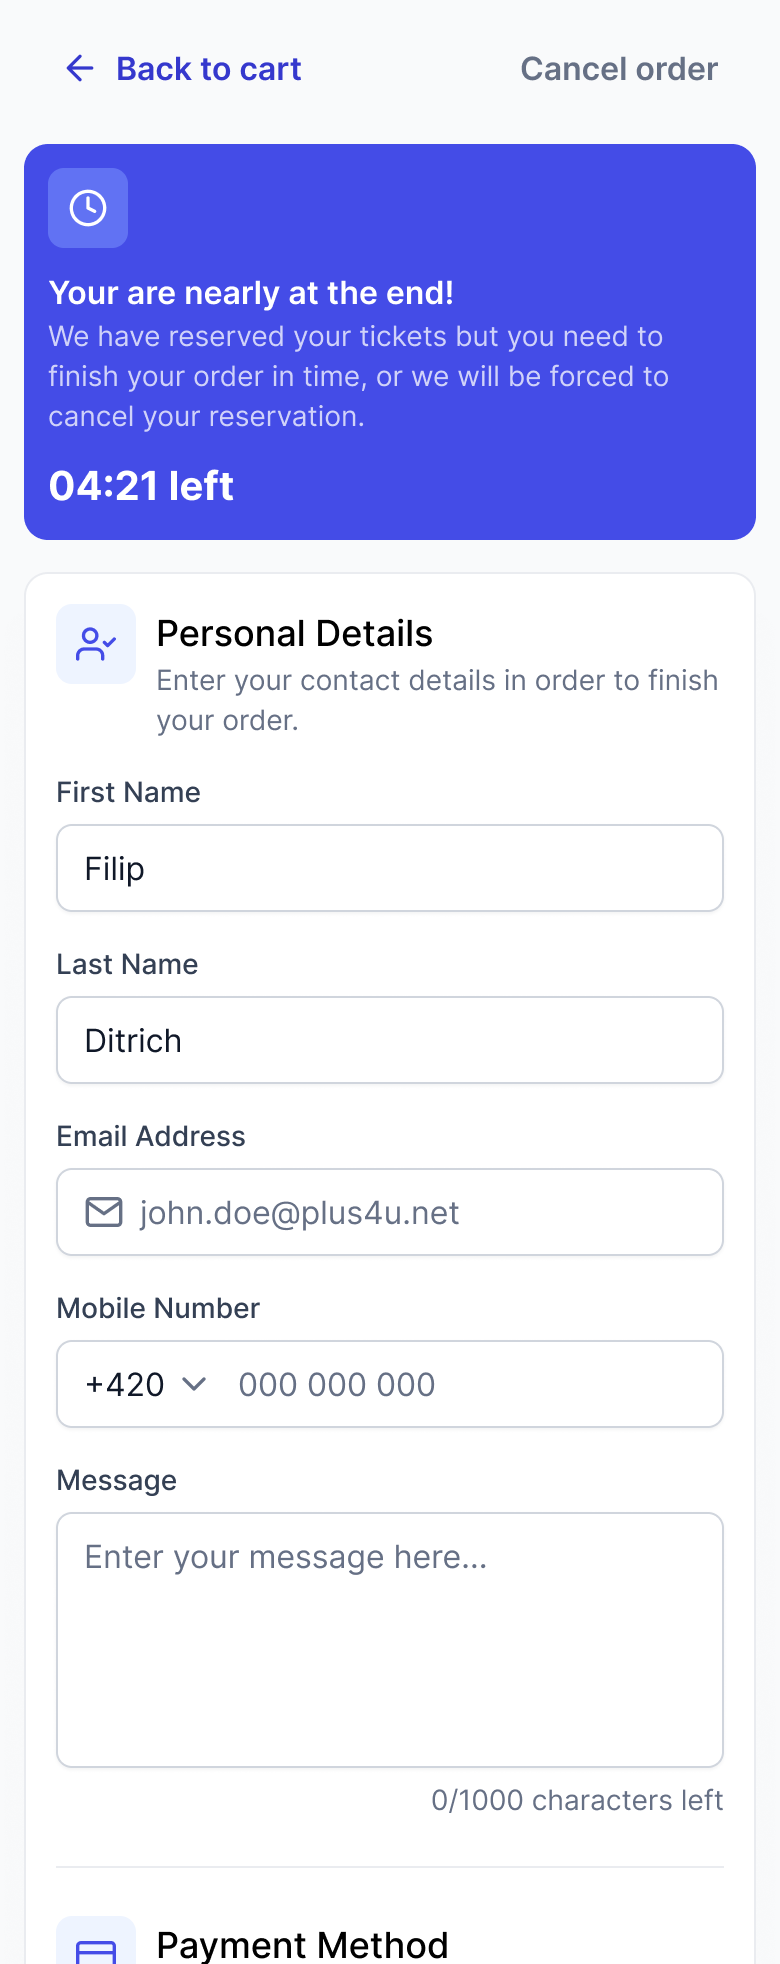
\includegraphics[width=\textwidth]{\FIGDIR/ui/us4-cart-checkout-mobile-1}
            \label{fig:us4-cart-checkout-mobile-1}
        \end{subfigure}
        \hfill
        \begin{subfigure}{0.4\textwidth}
            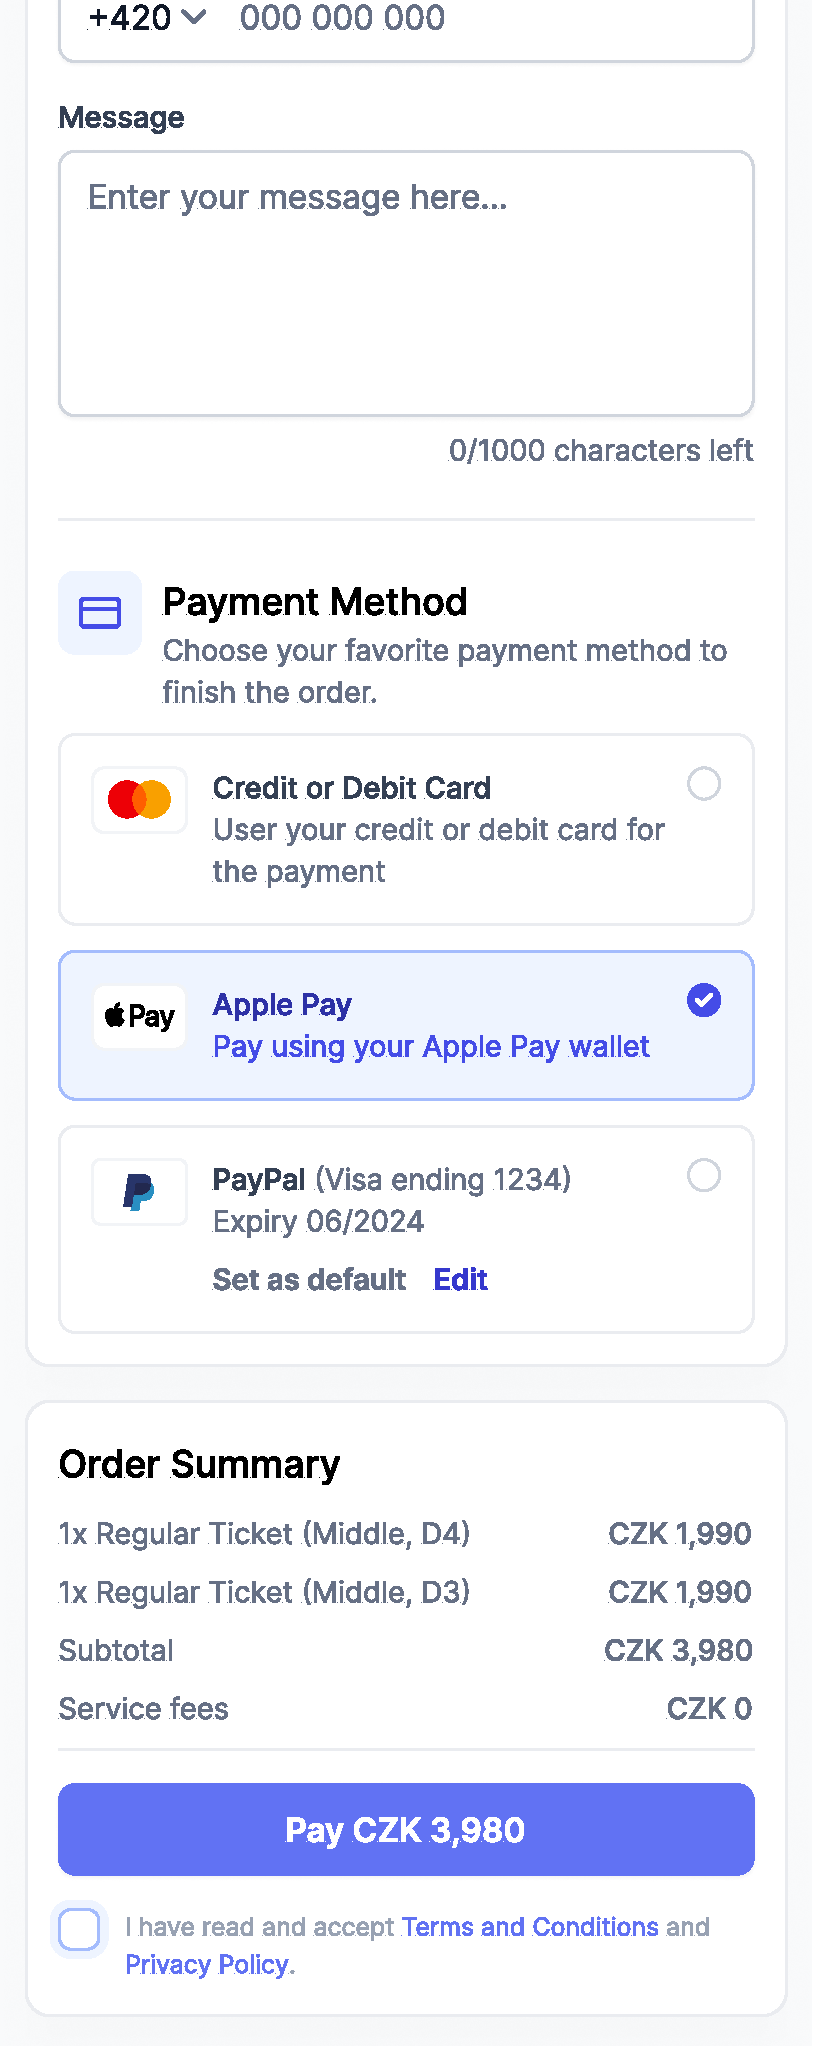
\includegraphics[width=\textwidth]{\FIGDIR/ui/us4-cart-checkout-mobile-2}
            \label{fig:us4-cart-checkout-mobile-2}
        \end{subfigure}

        \caption{Návrh komponent dokončení objednávky (mobilní verze)}
        \label{fig:us4-cart-checkout-mobile}
    \end{figure}

    V obou případech je proces vyřízení objednávky zakončen kliknutím na intuitivní tlačítko \foreign{Pay}.
    Byť není v rámci této práce nutné, v reálném nasazení by bylo nutné vyzvat zákazníka před dokončením objednávky k přečtení a potvrzení obchodních podmínek, případně dalších informací, které by mohly být pro zákazníka důležité.
    Proto je pod tlačítkem dokončení objednávky zobrazeno i povinné zaškrtávací políčko s přijetím obchodních podmínek, jak je zobrazeno na obrázku~\ref{fig:us4-cart-checkout-desktop} výše či v nejspodnější části obrázku~\ref{fig:us4-cart-checkout-mobile-2}.

    Po kliku na tlačítko dokončení objednávky by byl v reálném světe zákazník přesměrován k zaplacení objednávky, dle jeho zvolené platební metody.
    V rámci této práce je však tento krok zjednodušen a zákazník je přesměrován na stránku s potvrzením dokončení objednávky.

    Tato stránka předpokládá zobrazení informací o zaplacené objednávce a dalšími užitečnými kroky pro zákazníka.
    Vrchní část této komponenty zobrazuje jasné potvrzení o dokončení objednávky a jejím zaplacení spolu s možností stažení PDF souboru s potvrzením o jejím zaplacení, jak je zobrazeno na obrázku~\ref{fig:us4-order-confirmation-desktop} níže.

    \begin{figure}[H]
        \centering
        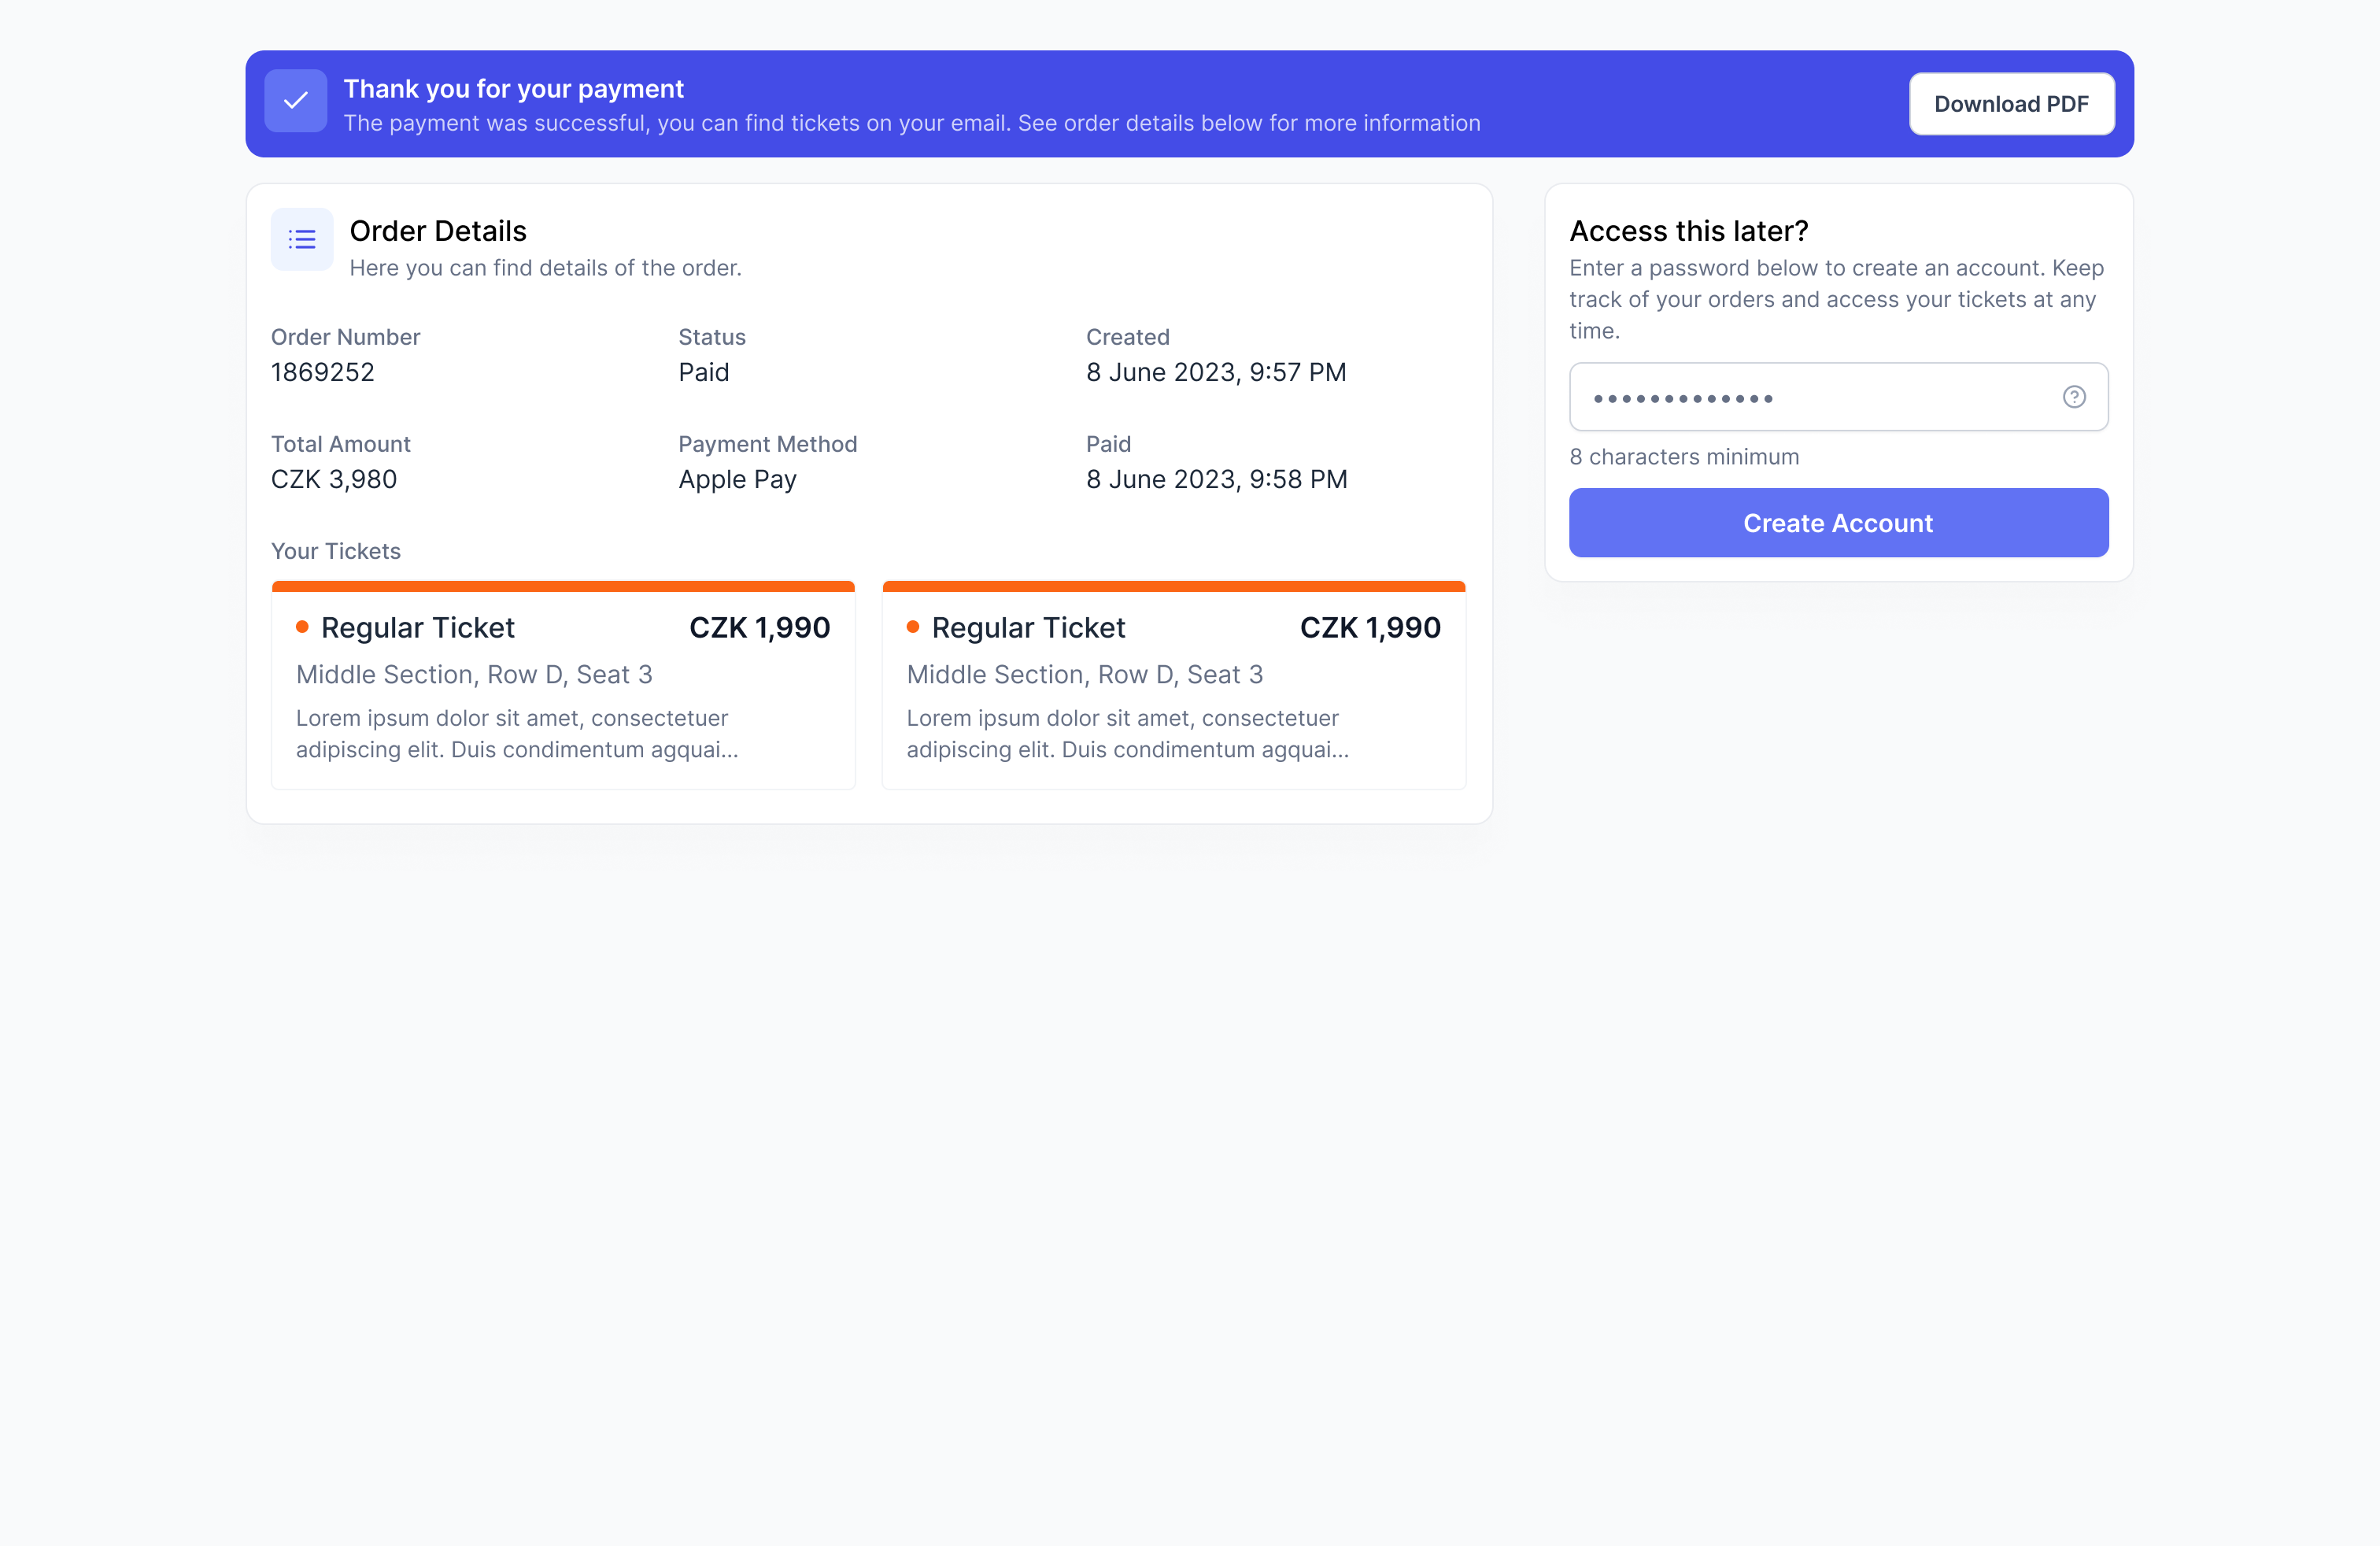
\includegraphics[width=\textwidth]{\FIGDIR/ui/us4-order-confirmation-desktop-1}
        \caption{Návrh komponent potvrzení objednávky (desktopová verze)}
        \label{fig:us4-order-confirmation-desktop}
    \end{figure}

    Dále je v rámci této komponenty zobrazen přehled dostupných informací o objednávce, jako je například číslo objednávky, datum a čas jejího vytvoření, stav, částka, informace o platbě či seznam zakoupených vstupenek a jejich míst.
    V tomto kroku, byť opět není nutnou součástí zadání této práce, by bylo užitečné zákazníka dále vybídnout z dokončení registrace a vytvoření účtu, aby mohl v budoucnu snadněji sledovat stav svých objednávek a měl přehled o svých vstupenkách.
    Tento krok je naznačen v pravém sloupci na obrázku~\ref{fig:us4-order-confirmation-desktop} výše, kde je zákazník vybídnut k vytvoření hesla pro svůj účet a tím tak vytvoření nového účtu.

    \begin{figure}[H]
        \centering
        \begin{subfigure}{0.4\textwidth}
            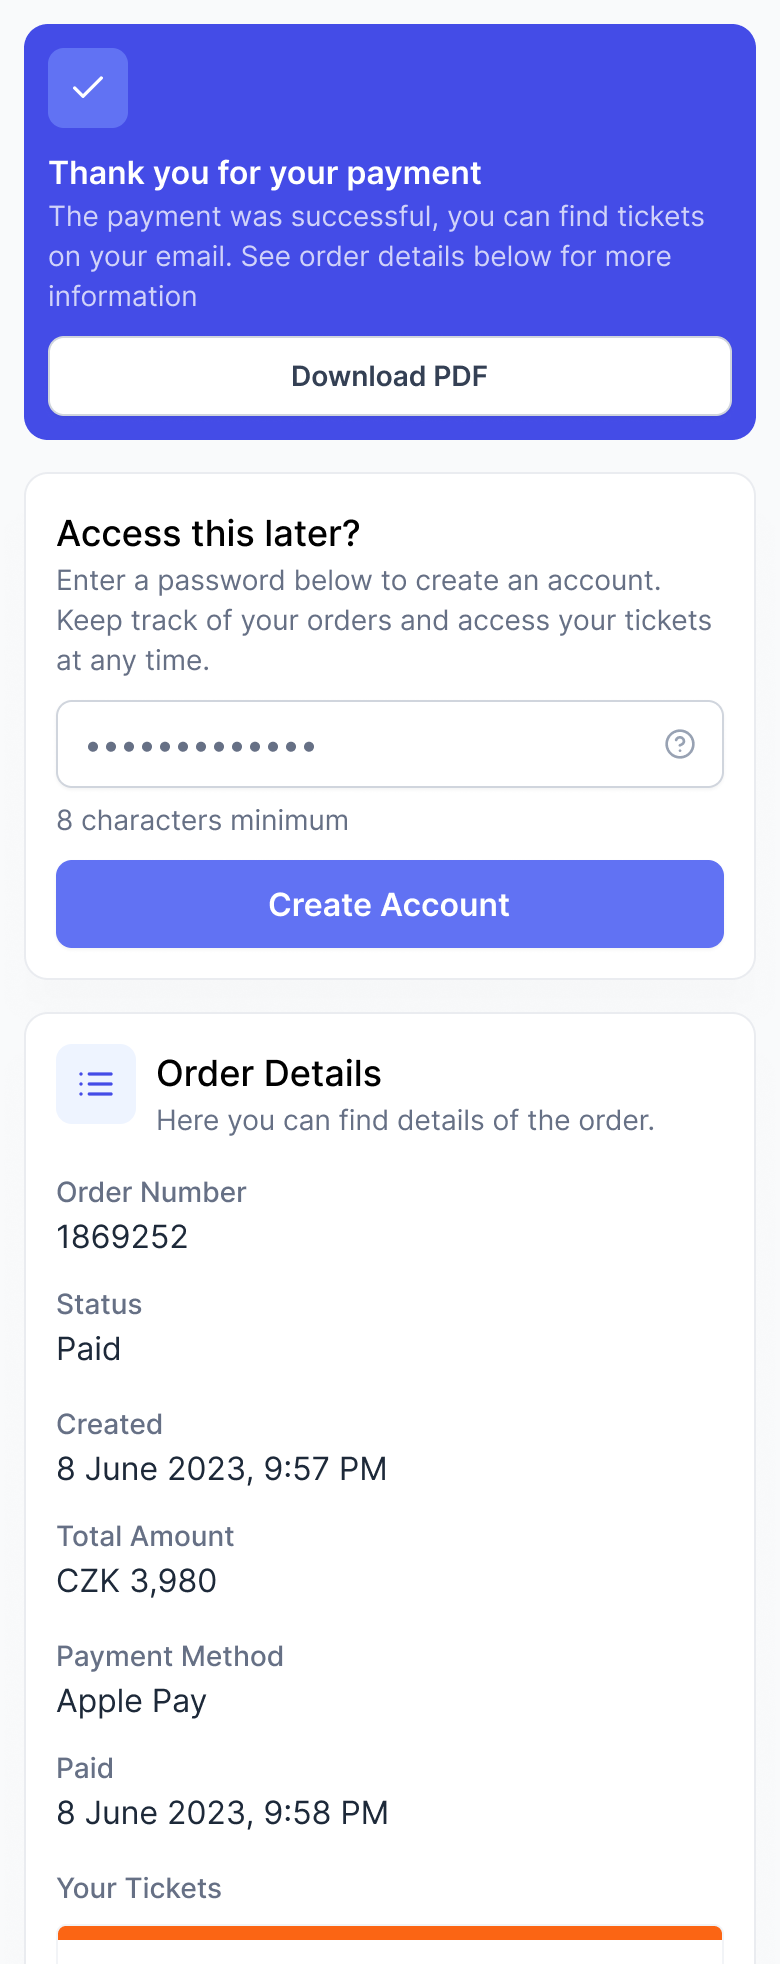
\includegraphics[width=\textwidth]{\FIGDIR/ui/us4-order-confirmation-mobile-1}
            \label{fig:us4-order-confirmation-mobile-1}
        \end{subfigure}
        \hfill
        \begin{subfigure}{0.4\textwidth}
            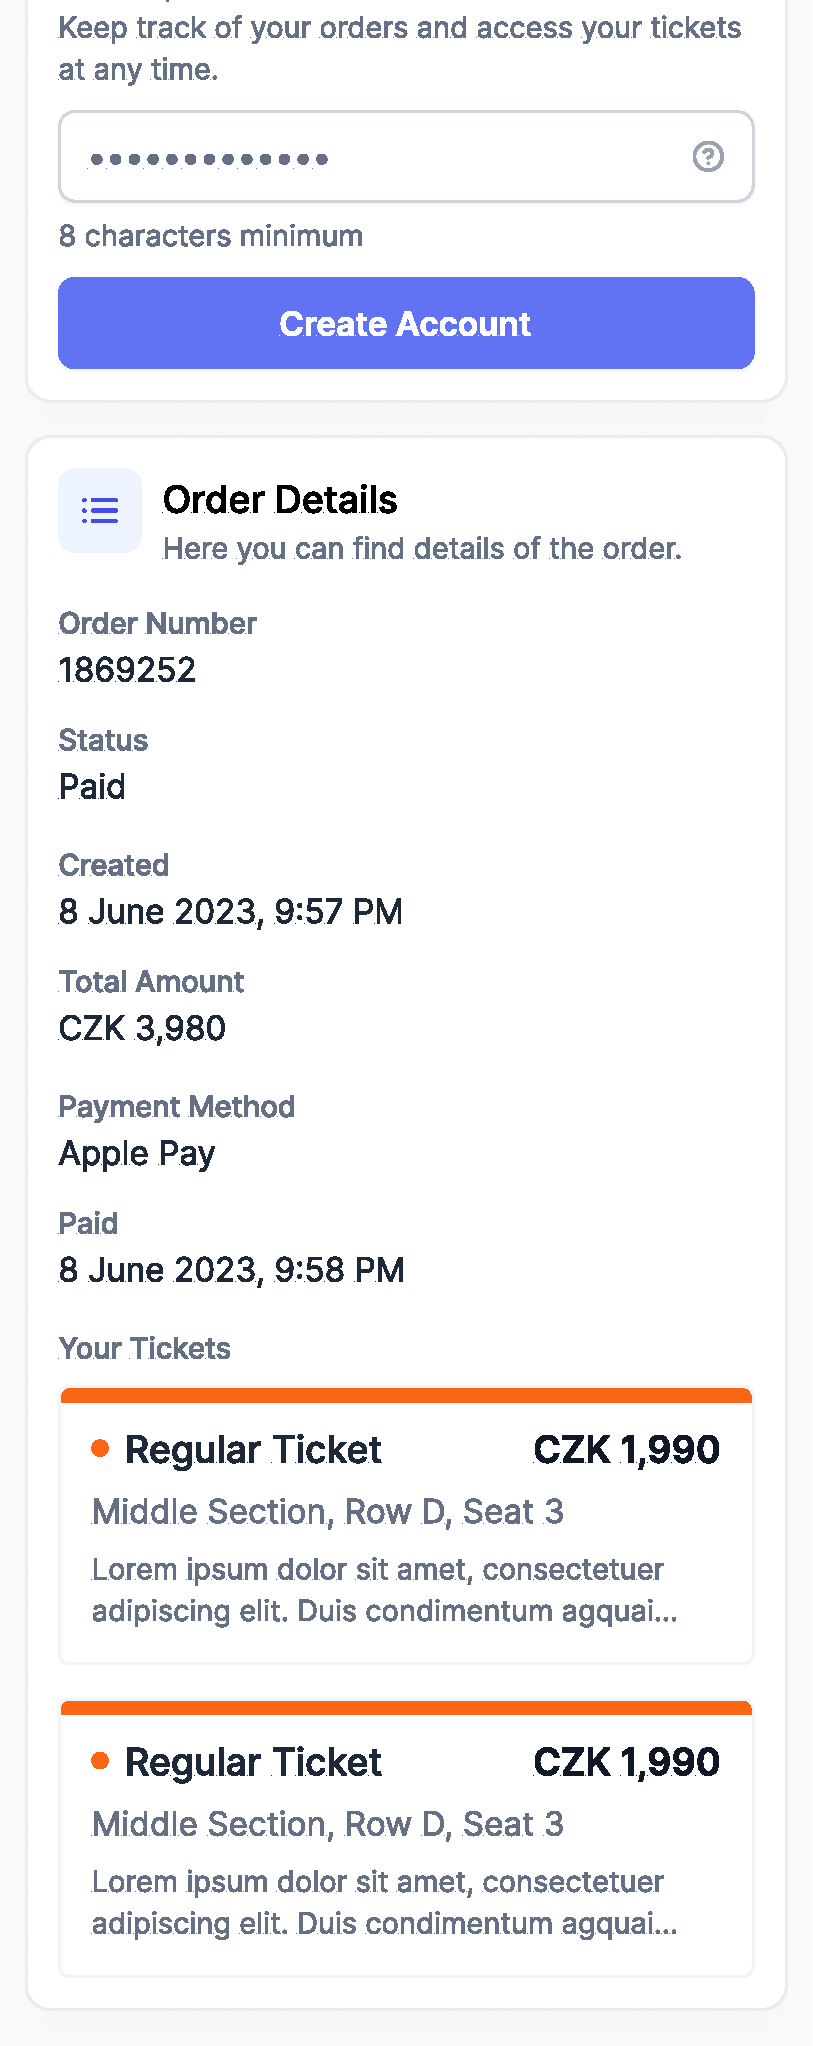
\includegraphics[width=\textwidth]{\FIGDIR/ui/us4-order-confirmation-mobile-2}
            \label{fig:us4-order-confirmation-mobile-2}
        \end{subfigure}

        \caption{Návrh komponent potvrzení objednávky (mobilní verze)}
        \label{fig:us4-order-confirmation-mobile}
    \end{figure}

    Mobilní rozložení této komponenty je opět pouze mírně upraveno, aby bylo možné všechny prvky zobrazit v jednom sloupci, jak je zobrazeno na obrázku~\ref{fig:us4-order-confirmation-mobile} výše.

    Tato kapitola vytvořila pevný základ pro pochopení návrhu uživatelského rozhraní, konkrétně v kontextu webového řešení pro prodej vstupenek s rezervací míst.
    To mj.\ zahrnovalo vytvoření uživatelských příběhů, jejich překlad do komponent uživatelského rozhraní a aplikaci efektivních principů návrhu uživatelského rozhraní.
    Dále bylo vyzdvihnut výběr nástroje Figma pro návrh těchto uživatelského rozhraní.

    V následující kapitole se pozornost přesouvá k implementaci těchto návrhů do funkčního online rezervačního systému s výběrem míst.
\end{subsection}
